\documentclass[11pt]{article}
\usepackage[a4paper,margin=2.5cm]{geometry}
\usepackage{amsmath,amssymb,amsthm,graphicx,booktabs,xcolor}
\usepackage[colorlinks=true,linkcolor=blue!60!black,citecolor=blue!60!black,urlcolor=blue!60!black]{hyperref}
\hypersetup{pdftitle={Holographic Entanglement of Fractal Regions},pdfauthor={Ruqing Chen}}
\newtheorem{theorem}{Theorem}
\newtheorem{proposition}{Proposition}[section]
\newtheorem{lemma}{Lemma}
\newtheorem{conjecture}{Conjecture}
\newtheorem{corollary}{Corollary}[section]
\theoremstyle{definition}\newtheorem{definition}{Definition}[section]
\theoremstyle{remark}\newtheorem*{remark}{Remark}

\graphicspath{{../figures/}{figures/}{./}}
\setlength{\emergencystretch}{3em}
\usepackage{xurl}
\newcommand{\cA}{\mathcal{A}}
\newcommand{\cD}{\mathfrak{D}}
\newcommand{\RR}{\mathbb{R}}
\newcommand{\ZZ}{\mathbb{Z}}
\newcommand{\TT}{\mathbb{T}}
\newcommand{\dd}{\mathrm{d}}
\newcommand{\Vol}{\mathrm{Vol}}
\newcommand{\Area}{\mathrm{Area}}
\newcommand{\GN}{G_N}

\title{Holographic Entanglement of Fractal Regions:\\
Complex Dimensions, Non-local Counterterms and Cosmic-Brane Multifractality}
\author{Ruqing Chen\\[2pt]
\small GUT Geoservice Inc., Montreal, Quebec, Canada\\
\small \href{mailto:ruqing@hotmail.com}{\texttt{ruqing@hotmail.com}}}
\date{\small DOI: \href{https://doi.org/10.5281/zenodo.23189575}{10.5281/zenodo.23189575}}

\begin{document}
\maketitle

\begin{abstract}
We study holographic entanglement entropy of boundary regions whose entangling surface is a
self-similar fractal of box dimension $D_\partial$. Using the Ryu--Takayanagi prescription in Poincar\'e
AdS$_{d+1}$ we show that the radial coordinate acts as a box-counting resolution: in the linearised
problem the bulk embedding is the boundary profile convolved with the positive kernel
$K_z(y)\propto z^d/(|y|^2+z^2)^{d-1}$, whose Fourier symbol is $(kz)^{d/2}K_{d/2}(kz)$. This yields the exact
identity $-\varepsilon\partial_\varepsilon S_A=(R/4\GN)\Vol(\gamma_A\cap\{z=\varepsilon\})$ and the scaling
$-\varepsilon\partial_\varepsilon S_A\asymp N_\varepsilon(\partial A)$.
For self-similar boundaries, bulk extensions of the boundary similarities imply a renewal equation whose
Mellin poles (complex dimensions) are the zeros of the Moran function; their imaginary parts form the
annihilator $\Lambda^\perp$ of the scaling group, and neither real nor imaginary parts are affected by
the bulk dynamics, which only enters the residues. Divergences are removed by the scale-non-local
counterterm $I_{ct}=-\frac{R}{4\GN}\int_{z_c}^{\infty}\frac{\dd z}{z}\,\Pi_{+}\Vol(\gamma_A\cap\{z\})$, and we show
why no counterterm of local multiplicative type can do so.
We further give a criterion for marginal complex dimensions. Combining Dong's thermodynamic reading of
the refined R\'enyi entropy with the multifractal formalism, we note that cosmic-brane areas equal the
singularity spectrum, $\tilde S_q=f(\alpha_q)\ln(1/\varepsilon)$, and that in Einstein gravity its shape is
fixed by the bulk. Finally, we propose a spectral fingerprint in lattice fractal-string resonators.
\end{abstract}

\tableofcontents

%=====================================================================
\section{Introduction}
\label{sec:intro}

The Ryu--Takayanagi (RT) formula~\cite{RT}
\begin{equation}
S_A=\frac{\Area(\gamma_A)}{4\GN}
\label{eq:RT}
\end{equation}
identifies the entanglement entropy of a boundary region $A$ with the area of the minimal bulk surface
$\gamma_A$ homologous to $A$. Nearly all explicit studies of~\eqref{eq:RT} concern regions with smooth
boundaries---balls, strips, and their small deformations---or boundaries with isolated singularities such as
corners and cones. In all these cases the ultraviolet structure of $S_A$ is controlled by a \emph{local}
expansion: the near-boundary Fefferman--Graham expansion of $\gamma_A$~\cite{FG,GW} determines the
divergent terms as integrals of local geometric invariants of $\partial A$, and holographic
renormalisation~\cite{Skenderis} removes them by local counterterms. The coefficient of the leading area-law
divergence is non-universal, while subleading logarithms (in even $d$, or from corners in $d=3$) carry
universal data of the CFT.

This locality rests on the entangling surface being smooth below some scale. A fractal entangling surface
has no such scale: structure is present at every resolution, and $\partial A$ has infinite
$(d-2)$-volume. Fractal boundaries arise naturally as coarse-grained interfaces, critical domain walls and
regions defined on fractal lattices, but the motivation here is structural. In holography the radial
coordinate $z$ geometrises the renormalisation group: the dilatation $(x,z)\mapsto(\lambda x,\lambda z)$ is an
isometry, and the bulk at depth $z$ encodes the boundary at resolution $z$. A fractal $\partial A$ is
therefore a probe of how the bulk organises an \emph{infinite hierarchy} of scales, and of how the continuous
dilatation symmetry of AdS interacts with the \emph{discrete} scale invariance (DSI) of a self-similar set.
We will see that this interaction has sharp consequences: complex scaling exponents, log-periodic terms, the
breakdown of local counterterms, and a precise dictionary between cosmic branes and multifractal spectra.

\paragraph{Prior work.}
Our analysis builds on several lines of work. The RT prescription~\cite{RT} was derived from the
gravitational path integral by Lewkowycz and Maldacena~\cite{LM}; Dong~\cite{Dong} extended the argument to
R\'enyi entropies, showing that the refined R\'enyi entropy is the area of a backreacting cosmic brane of
tension $T_q=(q-1)/(4q\GN)$. Explicit brane solutions for spherical regions are hyperbolic black
holes~\cite{HMSY}. Freedman and Headrick reformulated RT as a max-flow problem (``bit threads'')~\cite{FH};
explicit geodesic flows were constructed in~\cite{ABP}. Holography at a finite radial cutoff is related to
$T\bar T$-type deformations~\cite{MMV,HKST}. On the mathematical side, the theory of complex dimensions of
fractal strings and sets~\cite{LvF,LRZ} explains log-periodic oscillations in spectral and geometric
asymptotics through poles of zeta functions, the multifractal formalism~\cite{Halsey} describes measures with
a continuum of local scaling exponents, and DSI and its log-periodic signatures are reviewed in~\cite{Sornette}.
In two-dimensional CFT, the entanglement spectrum is known in closed form~\cite{CL,CT}.

Entanglement across fractal boundaries has been studied before, and our work builds directly on these
results. Hamma, Lidar and Severini showed that in the toric code the entanglement across a fractal boundary
of Hausdorff dimension $D$ obeys $S/p=\gamma\le1/D$~\cite{Hamma}. Faraji Astaneh computed the entanglement
entropy of regions on fractal spaces with heat-kernel methods for a free scalar~\cite{FarajiAstaneh}. He
found a leading divergence controlled by the spectral dimension and log-periodic corrections originating in
the complex dimensions of the fractal, including for a Cantor-string entangling boundary analysed with
Lapidus' zeta function, and he proposed a hyperscaling-violating holographic description. Akal found
log-periodic corrections for boundaries with the structure of finitely ramified self-similar
graphs~\cite{Akal}. Log-periodic entanglement also arises in aperiodic spin chains~\cite{IJZ,JZ}, and
generalised area laws governed by the boundary dimension have been observed on fractal
lattices~\cite{Hamma,FractalLattices}. Holographic entanglement for non-smooth entangling curves, including
singular points formed by logarithmic spirals, was studied in~\cite{HirataTakayanagi,MyersSingh,BMWK,Pastras},
and discrete scale invariance has been studied in holography from several angles~\cite{DSIholo,BDF,padic}.

\paragraph{Results.}
In contrast to~\cite{FarajiAstaneh}, where the space itself is fractal and the field theory is free, we keep
the bulk and the boundary smooth (Poincar\'e AdS dual to a CFT on $\RR^{d-1,1}$) and let only the entangling
surface be fractal, working throughout with the RT and cosmic-brane prescriptions. Within this setting our
results are:
\begin{enumerate}
\item \emph{Holographic box counting} (Theorem~\ref{thm:box}). The identity
$-\varepsilon\partial_\varepsilon S_A=(R/4\GN)\Vol(\gamma_A\cap\{z=\varepsilon\})$ holds exactly. In the
linearised problem the bulk acts on the boundary profile by an explicit positive smoothing kernel, and for a
Weierstrass-type boundary we prove $-\varepsilon\partial_\varepsilon S_A\asymp(R^{d-1}/4\GN)N_\varepsilon(\partial A)$
with $N_\varepsilon$ the box-counting function.
\item \emph{DSI locking} (Theorem~\ref{thm:dsi}). We adapt the renewal-theoretic proof of the
lattice/non-lattice dichotomy for Minkowski contents~\cite{LvF,Lalley,FalconerMink,Gatzouras} to the RT
cross-section content. The new inputs are the bulk extension of boundary similarities and a near-boundary
decoupling property (Lemma~\ref{lem:decoupling}). The complex dimensions governing $S_A$ are then the zeros
of the Moran function $1-\sum_j r_j^s$, and the bulk dynamics, linear or not, enters only through the
residues.
\item \emph{Non-local counterterm} (Proposition~\ref{prop:ct}). Building on the area renormalisation of
entangling surfaces~\cite{GW,TaylorWoodhead}, we construct the counterterm that renders $S_A$ finite. We show
(Proposition~\ref{prop:nolocal}) that local counterterms fail because cancellation requires inverting the
radial Euler operator $-z\partial_z$ on a lattice of complex exponents. This is related in spirit to the
scale-derivative refinement of Liu and Mezei~\cite{LiuMezei}.
\item \emph{Marginal complex dimensions} (Theorem~\ref{thm:marginal}). Within a distance-zeta
approximation, we give a necessary and sufficient condition for bounded log-periodic terms in the
renormalised entropy, together with an explicit lattice example.
\item \emph{Cosmic branes and multifractality} (Proposition~\ref{prop:brane}). Dong already noted that the
refined R\'enyi entropy is a thermodynamic entropy with respect to the modular
Hamiltonian~\cite{Dong,BeckSchlogl,Baez}. Combining this with the multifractal formalism gives
$\tilde S_q=f(\alpha_q)\ln(1/\varepsilon)$. The identity itself is elementary; its content is that in
Einstein gravity the shape of $f$ is fixed by the bulk, a consistency check that in $d=2$ reproduces the
known Calabrese--Lefevre spectrum~\cite{CL,CT}.
\item \emph{A spectral fingerprint} (Section~\ref{sec:exp}) of marginal complex dimensions, namely half-integer
log-harmonics, in lattice fractal-string resonators. It follows from the explicit formulas of fractal-string
spectral theory~\cite{LvF} and tests the zeta-function structure shared with our holographic analysis, not
holography itself.
\end{enumerate}
We are explicit about assumptions. Lemma~\ref{lem:decoupling} is proven in the linearised problem and
supported, but not proven, in the nonlinear one. Self-affine boundaries are not covered by
Theorem~\ref{thm:dsi}. The scale-transport equation of Section~\ref{sec:threads} is an organising conjecture.

\paragraph{Organisation.}
Section~\ref{sec:geometry} fixes conventions. Section~\ref{sec:arealaw} derives the fractal area law.
Section~\ref{sec:dsi} treats self-similar boundaries, complex dimensions and counterterms.
Section~\ref{sec:marginal} analyses marginal complex dimensions. Section~\ref{sec:renyi} turns to R\'enyi
entropies and cosmic branes. Section~\ref{sec:threads} discusses bit threads and scale transport, and
Section~\ref{sec:exp} the experimental fingerprint. We conclude in Section~\ref{sec:discussion}. Numerical
methods are collected in Appendix~\ref{app:numerics}.

%=====================================================================
\section{Geometry: Poincar\'e AdS and the radial resolution}
\label{sec:geometry}
% Christoffels, maximal-symmetry Riemann tensor, R=-d(d+1)/R^2 (SymPy-verified)
% Dimensional caveat: fractal curve needs CFT_3/AdS_4; AdS_5 uses curve x R (D_\partial=D+d-3)
We work on the $t=0$ slice of Poincar\'e AdS$_{d+1}$,
\begin{equation}
\dd s^2=\frac{R^2}{z^2}\left(\dd z^2+\dd x^2+\dd\vec y^{\,2}\right),\qquad \vec y\in\RR^{d-2},
\label{eq:slice}
\end{equation}
a copy of hyperbolic space $\mathbb H^d$. Boundary similarities $y\mapsto rOy+t$ extend to the bulk
isometries $(y,z)\mapsto(rOy+t,\,rz)$.

%=====================================================================
\section{Fractal area law}
\label{sec:arealaw}

\subsection{Setup}
Let $A\subset\RR^{d-1}$ be a region whose boundary $\partial A$ has upper and lower box (Minkowski) dimension
$D_\partial\in[d-2,d-1]$, defined through the box-counting function $N_\delta(\partial A)$, the minimal number
of $\delta$-cubes covering $\partial A$:
\begin{equation}
D_\partial=\lim_{\delta\to0}\frac{\ln N_\delta(\partial A)}{\ln(1/\delta)}.
\end{equation}
We use box rather than Hausdorff dimension throughout: it is the box-counting function that enters the
entropy, and the two dimensions coincide for the self-similar sets of Section~\ref{sec:dsi}.

For explicit computations we use \emph{graph-type} boundaries,
\begin{equation}
\partial A=\{x=f_0(y_1)\}\times[0,L_\perp]^{d-3},\qquad
f_0(y_1)=A_0\sum_{n\ge0}a^n\cos(k_0b^ny_1),\quad b>1,\ b^{-1}<a<1,
\label{eq:weierstrass}
\end{equation}
periodic in $y_1$ with period $Y=2\pi/k_0$ (we take $b$ integer). The graph of the Weierstrass function $f_0$
has box dimension $D=2+\ln a/\ln b\in(1,2)$~\cite{Falconer}, so $D_\partial=D+d-3$. For $d=3$ the entangling
surface is a fractal curve in the plane. Fractal curves therefore live naturally in CFT$_3$/AdS$_4$, while in
AdS$_5$ the construction~\eqref{eq:weierstrass} produces a fractal ``cylinder''.

\subsection{An exact radial identity}
Near the boundary we parametrise $\gamma_A$ as a graph $x=f(\vec y,z)$ over $(\vec y,z)$ for $z<z_0$. The induced
metric is $h_{ab}=(R^2/z^2)(\delta_{ab}+\partial_af\,\partial_bf)$ in coordinates $(\vec y,z)$, so
$\sqrt{h}=(R/z)^{d-1}\sqrt{1+|\partial f|^2}$ with $|\partial f|^2=|\nabla_yf|^2+f_z^2$. Define the
\emph{cross-section content}
\begin{equation}
\cA(z)=\int\dd^{d-2}y\,\sqrt{1+|\nabla_yf|^2+f_z^2}\,.
\label{eq:content}
\end{equation}
\begin{lemma}[Radial identity]
\label{lem:radial}
With a radial cutoff at $z=\varepsilon<z_0$,
\begin{equation}
\begin{gathered}
\Area_\varepsilon(\gamma_A)=\Area(\gamma_A\cap\{z>z_0\})+R^{d-1}\int_\varepsilon^{z_0}\dd z\,z^{1-d}\cA(z),\\
-\varepsilon\,\partial_\varepsilon S_A=\frac{R}{4\GN}\Vol\big(\gamma_A\cap\{z=\varepsilon\}\big),
\end{gathered}
\label{eq:radial}
\end{equation}
where $\Vol(\gamma_A\cap\{z=\varepsilon\})=(R/\varepsilon)^{d-2}\cA(\varepsilon)$ is the proper
$(d-2)$-volume of the cross-section.
\end{lemma}
\begin{proof}
The first equation is the area integral in the coordinates above. The second follows by differentiation:
$-\varepsilon\partial_\varepsilon\Area_\varepsilon=R^{d-1}\varepsilon^{2-d}\cA(\varepsilon)=R\,(R/\varepsilon)^{d-2}\cA(\varepsilon)$.
\end{proof}
Lemma~\ref{lem:radial} is exact and independent of any fractal structure; it is an immediate consequence
of RT in Poincar\'e coordinates, and the interpretation of the scale dependence of entanglement entropy as an
RG flow goes back to~\cite{LiuMezei}. The physics lies entirely in the small-$z$ behaviour of $\cA(z)$,
which we now determine.

\subsection{The linearised problem and the radial kernel}
Varying the area functional gives the RT equation
\begin{equation}
\partial_z\!\left(\frac{z^{1-d}f_z}{\sqrt{1+|\partial f|^2}}\right)+\nabla_y\!\cdot\!\left(\frac{z^{1-d}\nabla_yf}{\sqrt{1+|\partial f|^2}}\right)=0,
\label{eq:RTeq}
\end{equation}
whose linearisation about the plane $f=0$, standard in studies of the shape dependence of holographic
entanglement~\cite{Mezei,AllaisMezei}, is
\begin{equation}
f_{zz}-\frac{d-1}{z}f_z+\nabla_y^2f=0,\qquad f(\vec y,0)=f_0(\vec y).
\label{eq:linRT}
\end{equation}
For a Fourier mode $f=\varphi(z)e^{ik\cdot y}$, \eqref{eq:linRT} becomes the modified Bessel equation in the
variable $x=|k|z$ after the substitution $\varphi=x^{\nu}u(x)$, $\nu=d/2$. Its solution decaying as
$z\to\infty$ and normalised by $\varphi(0)=1$ is
\begin{equation}
\phi_d(x)=\frac{x^{\nu}K_\nu(x)}{2^{\nu-1}\Gamma(\nu)},\qquad \nu=\frac d2 .
\label{eq:phi}
\end{equation}
For $d=3$ it is elementary, $\phi_3(x)=(1+x)e^{-x}$. The two regimes of~\eqref{eq:phi} follow from the
standard expansions of $K_\nu$:
\begin{align}
\phi_d(x)&=1-\frac{x^2}{2(d-2)}+\dots+c_d\,x^{d}\,(1+O(x^2))\ [\times\ln x \text{ for even } d],
&& x\to0,\label{eq:phismall}\\
\phi_d(x)&=\frac{\sqrt{\pi/2}}{2^{\nu-1}\Gamma(\nu)}\,x^{\frac{d-1}{2}}e^{-x}\big(1+O(x^{-1})\big),
&& x\to\infty.\label{eq:philarge}
\end{align}
The small-$x$ expansion follows from $K_\nu=\frac{\pi}{2}\frac{I_{-\nu}-I_\nu}{\sin\nu\pi}$ and the
reflection formula $\Gamma(\nu)\Gamma(1-\nu)=\pi/\sin\nu\pi$. The large-$x$ form is Hankel's asymptotic
expansion. Thus features of wavenumber $k$ are transmitted essentially unchanged to depth $z\ll1/k$ and are
exponentially suppressed for $z\gg1/k$. The first non-local datum enters at order $x^d$, the normalisable
mode.

\begin{proposition}[Radial smoothing kernel]
\label{prop:kernel}
The solution of~\eqref{eq:linRT} is $f(\cdot,z)=K_z*f_0$ with
\begin{equation}
K_z(\vec y)=\frac{\Gamma(d-1)}{\pi^{\frac{d-2}{2}}\Gamma(\frac d2)}\;\frac{z^d}{(|\vec y|^2+z^2)^{d-1}},
\qquad \int_{\RR^{d-2}}K_z=1,\qquad K_z>0 .
\label{eq:kernel}
\end{equation}
\end{proposition}
\begin{proof}
In $\RR^n$ the Fourier transform of $(1+|y|^2)^{-a}$ is proportional to $|k|^{a-n/2}K_{a-n/2}(|k|)$. With
$n=d-2$ and $a=d-1$ we get $a-n/2=d/2=\nu$, which matches~\eqref{eq:phi} after rescaling $y\to y/z$.
Dimensional analysis fixes the power $z^d$, and the normalisation follows from $\phi_d(0)=1$. For $d=3$ one
checks directly that $(1-z\partial_z)\frac{z}{\pi(y^2+z^2)}=\frac{2z^3}{\pi(y^2+z^2)^2}$, the image of
$e^{-|k|z}(1+|k|z)$.
\end{proof}
The kernel~\eqref{eq:kernel} makes the slogan ``radial depth $=$ resolution'' precise. The linearised RT surface
at depth $z$ is the boundary profile averaged with a positive, unit-mass kernel of width $z$, and its tail
$\int_{|y|>\ell}K_z=O((z/\ell)^{d})$ quantifies how weakly distant boundary data influence the surface. This
is the basis of Lemma~\ref{lem:decoupling} below.

\subsection{Content asymptotics for Weierstrass boundaries}
Write $x=k_0z$ and $k_n=k_0b^n$. For~\eqref{eq:weierstrass}, orthogonality of the Fourier modes on one period
gives
\begin{equation}
\|\partial_{y_1}f(\cdot,z)\|_{L^2}^2=\frac{Y}{2}A_0^2k_0^2\sum_{n\ge0}(ab)^{2n}\phi_d(b^nx)^2,\qquad
\|f_z(\cdot,z)\|_{L^2}^2=\frac{Y}{2}A_0^2k_0^2\sum_{n\ge0}(ab)^{2n}\phi_d'(b^nx)^2 .
\label{eq:L2}
\end{equation}
Since $a=b^{D-2}$, the growth factor is $ab=b^{D-1}>1$.
\begin{lemma}[Log-periodic sums]
\label{lem:logper}
Let $h\ge0$ be continuous on $(0,\infty)$, bounded near $0$, decaying exponentially at $\infty$, and not
identically zero. Then
\begin{equation}
\Psi_h(x):=\sum_{n\in\ZZ}(ab)^{2n}h(b^nx)=x^{-2(D-1)}P_h(\log_bx),
\end{equation}
with $P_h$ continuous, 1-periodic and strictly positive. The one-sided sum over $n\ge0$ differs from
$\Psi_h$ by $O(1)$ as $x\to0$.
\end{lemma}
\begin{proof}
The sum converges because $(ab)^{2n}\to0$ for $n\to-\infty$, where $h$ is bounded, and because $h$ decays
exponentially for $n\to+\infty$. Shifting the summation index gives $\Psi_h(bx)=(ab)^{-2}\Psi_h(x)=b^{-2(D-1)}\Psi_h(x)$,
so $x^{2(D-1)}\Psi_h(x)$ is invariant under $x\mapsto bx$, i.e.\ periodic in $\log_bx$. It is continuous,
and positive because some term is positive. The terms with $n<0$ sum to at most $\sup h\,\sum_{n<0}(ab)^{2n}<\infty$.
\end{proof}
Applying Lemma~\ref{lem:logper} with $h=\phi_d^2$ and $h=\phi_d'^2$ gives
$\|\partial_{y_1}f\|_{2},\|f_z\|_{2}\asymp z^{1-D}$ as $z\to0$. To control $\cA$, which involves $L^1$
norms, we use that both $\partial_{y_1}f(\cdot,z)$ and $f_z(\cdot,z)$ are \emph{Hadamard-lacunary}
trigonometric series in $y_1$ (frequency ratio $b>1$). For such series all $L^p$ norms, $p<\infty$, are
equivalent with constants depending only on $b$~\cite{Zygmund}:
$B_b\|g\|_2\le\|g\|_1\le\sqrt{Y}\|g\|_2$.
\begin{proposition}[Content bounds]
\label{prop:content}
For the linearised RT surface of~\eqref{eq:weierstrass} there are constants $0<c_1\le c_2$ and $z_*>0$ such
that
\begin{equation}
c_1\,z^{(d-2)-D_\partial}\le\cA(z)\le c_2\,z^{(d-2)-D_\partial},\qquad 0<z\le z_*.
\label{eq:contentbounds}
\end{equation}
\end{proposition}
\begin{proof}
From $\max(1,|\partial_{y_1}f|)\le\sqrt{1+|\partial f|^2}\le1+|\partial_{y_1}f|+|f_z|$ and integration over a
period,
$L_\perp^{d-3}\max(Y,\|\partial_{y_1}f\|_1)\le\cA\le L_\perp^{d-3}(Y+\|\partial_{y_1}f\|_1+\|f_z\|_1)$.
Lacunarity and Lemma~\ref{lem:logper} turn both bounds into $\asymp z^{1-D}$ once $z^{1-D}\gg1$. Finally,
$z^{1-D}L_\perp^{d-3}\asymp z^{(d-2)-D_\partial}$ in units where the transverse box count is
$(L_\perp/z)^{d-3}$.
\end{proof}

\subsection{Holographic box counting}
\begin{theorem}[Holographic box counting]
\label{thm:box}
Let $\gamma_A$ be the RT surface of $A$ and $\cA$ its cross-section content~\eqref{eq:content}.
\begin{enumerate}
\item[(i)] (Exact.) $-\varepsilon\partial_\varepsilon S_A=\frac{R}{4\GN}\Vol(\gamma_A\cap\{z=\varepsilon\})=\frac{R^{d-1}}{4\GN}\varepsilon^{2-d}\cA(\varepsilon)$.
\item[(ii)] (Scaling.) If~\eqref{eq:contentbounds} holds with $D_\partial>0$, then
\begin{equation}
\frac{R^{d-1}c_1}{4\GN D_\partial}\varepsilon^{-D_\partial}(1+o(1))\le S_A\le\frac{R^{d-1}c_2}{4\GN D_\partial}\varepsilon^{-D_\partial}(1+o(1)).
\end{equation}
\item[(iii)] (Log-periodic refinement.) If $z^{D_\partial-(d-2)}\cA(z)=P(\ln z)+o(1)$ with $P$ continuous and
periodic of period $\ln b$, $P(t)=\sum_mP_me^{2\pi imt/\ln b}$, then
\begin{equation}
\begin{gathered}
S_A=\frac{R^{d-1}}{4\GN}\,\varepsilon^{-D_\partial}\tilde P(\ln\varepsilon)+o(\varepsilon^{-D_\partial}),\\
\tilde P(t)=\int_0^\infty e^{-D_\partial u}P(t+u)\,\dd u,\qquad \tilde P_m=\frac{P_m}{D_\partial-2\pi im/\ln b}.
\end{gathered}
\label{eq:Ptilde}
\end{equation}
In particular, the mean coefficient is reduced by $1/D_\partial$ relative to the smooth-boundary normalisation.
(A factor $1/D$ also appears in the toric-code bound of~\cite{Hamma}, for different reasons.)
\item[(iv)] (Box counting.) For the linearised Weierstrass model, $\cA(\varepsilon)\asymp\varepsilon^{d-2}N_\varepsilon(\partial A)$, hence
\begin{equation}
-\varepsilon\,\partial_\varepsilon S_A\asymp\frac{R^{d-1}}{4\GN}\,N_\varepsilon(\partial A).
\label{eq:boxcount}
\end{equation}
\end{enumerate}
\end{theorem}
\begin{proof}
(i) is Lemma~\ref{lem:radial}. For (ii), insert~\eqref{eq:contentbounds} into~\eqref{eq:radial}: the
integral $R^{d-1}\int_\varepsilon^{z_*}z^{1-d}z^{(d-2)-D_\partial}\dd z=R^{d-1}(\varepsilon^{-D_\partial}-z_*^{-D_\partial})/D_\partial$,
and the remaining contributions are $\varepsilon$-independent. For (iii), substitute $z=\varepsilon e^u$:
$\int_\varepsilon z^{-1-D_\partial}P(\ln z)\dd z=\varepsilon^{-D_\partial}\int_0^\infty e^{-D_\partial u}P(\ln\varepsilon+u)\dd u$, and the
$o(1)$ remainder contributes $o(\varepsilon^{-D_\partial})$. Mode by mode,
$\int_0^\infty e^{-D_\partial u}e^{i\omega(t+u)}\dd u=e^{i\omega t}/(D_\partial-i\omega)$. For (iv), the box-counting
function of the graph of $f_0$ satisfies $N_\delta\asymp\delta^{-D}$~\cite{Falconer}, so
$N_\varepsilon(\partial A)\asymp\varepsilon^{-D}(L_\perp/\varepsilon)^{d-3}$. Comparing with
Proposition~\ref{prop:content} and (i) gives~\eqref{eq:boxcount}.
\end{proof}

\begin{remark}
In the linearised model, \eqref{eq:L2} and Lemma~\ref{lem:logper} show that the $L^2$ content is
\emph{exactly} log-periodic up to $O(1)$, and the hypothesis of (iii) holds for $\|\nabla f\|_2^2$. For the
$L^1$ content $\cA$ itself, the hypothesis of (iii) follows from the renewal structure established in
Section~\ref{sec:dsi}. Linearisation is not uniformly controlled at small $z$, since slopes grow like
$z^{1-D}$. For self-similar boundaries, however, Section~\ref{sec:dsi} shows that the scaling of $\cA$ is
fixed by symmetry independently of linearisation.
\end{remark}

\subsection{Numerical test}
\label{sec:table1}
We computed $\cA(z)$ for the linearised surface with $b=3$, six modes, $A_0=k_0=1$ and $d=3$, on $2^{15}$
points per period, and fitted power laws over the window $3/k_{\max}\le z\le0.3/k_0$ (about $2.4$ decades).
The results are in Table~\ref{tab:exponents} and Fig.~\ref{fig:scaling}.
\begin{table}[htbp]
\centering
\begin{tabular}{ccccc}
\toprule
$D$ & $\cA$ exponent (num.) & $1-D$ & $S_A$ exponent (num.) & $-D$\\
\midrule
1.1 & $-0.114$ & $-0.100$ & $-1.154$ & $-1.100$\\
1.3 & $-0.248$ & $-0.300$ & $-1.260$ & $-1.300$\\
1.5 & $-0.439$ & $-0.500$ & $-1.422$ & $-1.500$\\
1.7 & $-0.654$ & $-0.700$ & $-1.621$ & $-1.700$\\
1.9 & $-0.871$ & $-0.900$ & $-1.836$ & $-1.900$\\
\bottomrule
\end{tabular}
\caption{Fitted scaling exponents of the cross-section content and of the regulated entropy (linearised
Weierstrass model, $d=3$, $b=3$, six modes) against the predictions of Theorem~\ref{thm:box}.}
\label{tab:exponents}
\end{table}

The deviations, $0.03$--$0.08$, are systematic rather than statistical, and four effects account for them.
\emph{(a) The smooth pole.} The content contains a constant term $c_s$ (the ``1'' under the square root,
i.e.\ the exponent $\omega=d-2$ of a smooth boundary). A pure power-law fit absorbs it and underestimates
$|1-D|$, as seen in the $\cA$ column. The bias is largest when the two exponents are close; for $D=1.1$ the
model is moreover pre-asymptotic, since $ab=3^{0.1}$ makes the slopes $O(1)$ throughout the window.
\emph{(b) Infrared subtraction.} The regulated entropy is $C\varepsilon^{-D}-C'$ with $C'>0$ from the upper
limit of the window. Its logarithmic slope, $-D/(1-(C'/C)\varepsilon^{D})$, is steeper than $-D$, which
explains the steeper entropy exponents at small $D$.
\emph{(c) Log-periodic modulation.} Its relative amplitude is about $1\%$ (Section~\ref{sec:dsi}). Over a
window of about four periods this biases a straight-line fit at the $10^{-3}$ level, a subdominant effect.
\emph{(d) Truncation and non-homogeneity.} With finitely many modes the content saturates below
$z\sim1/k_{\max}$, and the integrand $\sqrt{1+|\partial f|^2}$ restores exact affine scaling only for
$|\partial f|\gg1$.
Including the smooth pole and three log-periodic harmonics in the fit (Section~\ref{sec:dsinum}) reduces
the discrepancy at $D=1.5$ from $0.061$ to $0.024$, with relative residual $1.5\times10^{-3}$.

\begin{figure}[htbp]
\centering
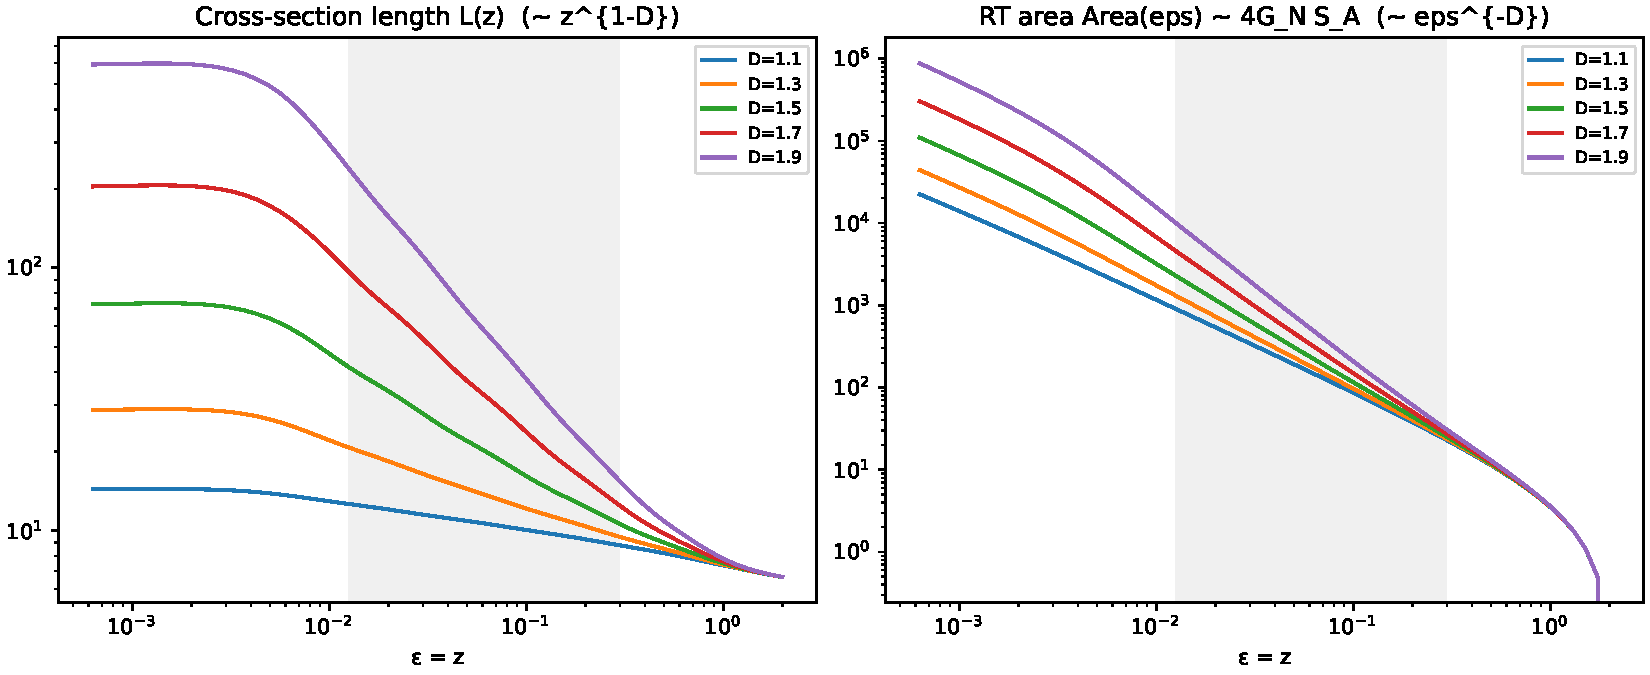
\includegraphics[width=0.9\textwidth]{rt_scaling}
\caption{Cross-section content $\cA(z)$ (left) and regulated RT area (right) for the linearised Weierstrass
model. The shaded band marks the fit window.}
\label{fig:scaling}
\end{figure}

%=====================================================================
\section{Discrete scale invariance and complex dimensions}
\label{sec:dsi}

\subsection{Self-similar boundaries and the bulk similarity group}
\begin{definition}
Let $\{S_j\}_{j=1}^N$ be similarities of $\RR^{d-1}$, $S_j(y)=r_jO_jy+t_j$ with $0<r_j<1$ and
$O_j\in O(d-1)$, satisfying the open set condition. Their attractor $K=\bigcup_jS_j(K)$ has box and
Hausdorff dimension equal to the similarity dimension $D_\partial$, the unique real solution of
$\sum_jr_j^{D_\partial}=1$~\cite{Hutchinson,Falconer}. Set $\lambda_j=\ln(1/r_j)$ and let
$\Lambda\subset(\RR,+)$ be the subgroup generated by $\{\lambda_j\}$. The system is \emph{lattice} if
$\Lambda=(\ln b)\ZZ$ for some $b>1$, and \emph{non-lattice} otherwise, in which case $\Lambda$ is dense.
\end{definition}

\begin{lemma}[Bulk extension]
\label{lem:extension}
Each $S_j$ extends to the isometry $\hat S_j(y,z)=(S_j(y),r_jz)$ of~\eqref{eq:slice}. If $\gamma$ is the RT
surface of a region $B$, then $\hat S_j(\gamma)$ is the RT surface of $S_j(B)$, and the cross-section
contents satisfy $\cA_{\hat S_j(\gamma)}(z)=r_j^{d-2}\cA_\gamma(z/r_j)$.
\end{lemma}
\begin{proof}
The metric $R^2(\dd z^2+\dd y^2)/z^2$ is invariant under $(y,z)\mapsto(rOy+t,rz)$. Isometries preserve areas and
homology, hence minimality. The cross-section of $\hat S_j(\gamma)$ at depth $z$ is the image of the
cross-section of $\gamma$ at depth $z/r_j$ under $S_j$, whose coordinate $(d-2)$-volume scales by
$r_j^{d-2}$.
\end{proof}

\subsection{Near-boundary decoupling}
\begin{lemma}[Near-boundary decoupling]
\label{lem:decoupling}
There exist $\eta>0$ and $C<\infty$ with the following property. If two regions $A,A'$ coincide in a ball
$B_\ell(p)$, then for $z\le\ell$ the cross-section contents of $\gamma_A$ and $\gamma_{A'}$ over $B_{\ell/2}(p)$
differ by at most $C(z/\ell)^{\eta}$ times either one.
\end{lemma}
We do not have a proof of Lemma~\ref{lem:decoupling} for the nonlinear problem with fractal data. Three
independent lines of evidence support it.
\begin{enumerate}
\item \emph{Linearised problem (proven).} By Proposition~\ref{prop:kernel}, a change of boundary data outside
$B_\ell(p)$ alters $f$ at $(y,z)$, $y\in B_{\ell/2}(p)$, by at most $\|\delta f_0\|_\infty\int_{|y'|>\ell/2}K_z$,
which is $O((z/\ell)^d)$. Hence $\eta=d$.
\item \emph{Fefferman--Graham structure (smooth case).} For smooth $\partial A$ the embedding of an extremal
surface has the near-boundary expansion
$X^i(\sigma,z)=X^i_0(\sigma)+z^2X^i_2(\sigma)+\dots+z^dX^i_d(\sigma)+\dots$, with logarithms for even $d$. Here
$X_2^i\propto K^i$ (the trace of the extrinsic curvature of $\partial A$) and all coefficients below
$X_d$ are local functionals of $\partial A$~\cite{GW}. $X_d$ is the first coefficient not fixed by local
data, so non-local information enters at relative order $z^d$, consistent with $\eta=d$.
\item \emph{Comparison principle.} By entanglement wedge nesting~\cite{Wall}, $\gamma_{A\cap A'}$ and
$\gamma_{A\cup A'}$ bound $\gamma_A$ and $\gamma_{A'}$ from either side. Nesting confines the deviation
qualitatively; a quantitative estimate would require barrier surfaces controlled near the boundary.
\end{enumerate}
For fractal $\partial A$ the Fefferman--Graham expansion does not apply (curvatures are unbounded), and in
the nonlinear problem $\eta$ need not equal $d$. Theorem~\ref{thm:dsi} only uses $\eta>0$.

\subsection{DSI locking}
The mathematical core of the following theorem is not new. That the complex dimensions of a self-similar
set are the zeros of the Moran function, and that its Minkowski content is log-periodic in the lattice case
and converges in the non-lattice case, is due to Lapidus and van Frankenhuijsen, Falconer, Gatzouras and
Lalley~\cite{LvF,FalconerMink,Gatzouras,Lalley,LvFsurvey}, and log-periodicity as a signature of DSI is
reviewed in~\cite{Sornette}. We adapt their renewal-theoretic argument to the RT cross-section content. The
new inputs are Lemma~\ref{lem:extension}, which transports the boundary self-similarity to the bulk, and
Lemma~\ref{lem:decoupling}, which controls the non-locality of the minimal-surface problem.

For a region $A$ with $\partial A=K$ and $z_0$ small, define the content zeta function
\begin{equation}
\zeta_{\cA}(s)=\int_0^{z_0}z^{\,s-(d-1)}\cA(z)\,\dd z,
\label{eq:zetaA}
\end{equation}
normalised so that a term $C\,z^{(d-2)-\omega}$ in $\cA$ produces a pole $C/(s-\omega)$. Set
\begin{equation}
M(s)=1-\sum_{j=1}^Nr_j^{\,s}.
\end{equation}

\begin{theorem}[DSI locking]
\label{thm:dsi}
Let $\partial A=K$ be a self-similar set as above, assume Lemma~\ref{lem:decoupling}, and let $\cA$ be
locally bounded. Then:
\begin{enumerate}
\item[(i)] $\zeta_\cA$ converges for $\mathrm{Re}\,s>D_\partial$ and continues meromorphically to
$\mathrm{Re}\,s>D_\partial-\eta'$ for some $\eta'>0$. There
\begin{equation}
\zeta_\cA(s)=\frac{\zeta_g(s)+E(s)}{M(s)},
\label{eq:zetafactor}
\end{equation}
with $E$ entire and $\zeta_g$ holomorphic. Its poles there lie in the zero set
$\cD=\{s:\ M(s)=0\}$.
\item[(ii)] On the line $\mathrm{Re}\,s=D_\partial$,
\begin{equation}
\cD\cap\{\mathrm{Re}\,s=D_\partial\}=D_\partial+i\Lambda^\perp,\qquad
\Lambda^\perp=\{t\in\RR:\ e^{it\lambda}=1\ \ \forall\lambda\in\Lambda\},
\end{equation}
so $\Lambda^\perp=(2\pi/\ln b)\ZZ$ in the lattice case and $\Lambda^\perp=\{0\}$ otherwise. All these zeros
are simple.
\item[(iii)] The location of the poles depends only on the scaling ratios $\{r_j\}$. The bulk dynamics, linear
or nonlinear, enters only through the residues
$C_m=\big(\zeta_g(s_m)+E(s_m)\big)/M'(s_m)$ at $s_m=D_\partial+i t_m$, $t_m\in\Lambda^\perp$.
\item[(iv)] In the lattice case, $z^{D_\partial-(d-2)}\cA(z)=P(\ln z)+o(1)$ with $P$ periodic of period
$\ln b$, whose Fourier frequencies lie in $\Lambda^\perp$. In the non-lattice case the limit is a constant.
\end{enumerate}
\end{theorem}

\begin{proof}
\emph{Step 1 (Renewal equation).} Decompose the near-boundary part of $\gamma_A$ into pieces lying over
neighbourhoods of $S_j(K)$. By Lemma~\ref{lem:extension}, the RT surface of $S_j(A)$ is $\hat S_j(\gamma_A)$.
Near $S_j(K)$ but away from the finitely many junction points where different copies meet, $A$ and $S_j(A)$
coincide in balls of radius comparable to the distance $\rho$ to the junctions. Lemma~\ref{lem:decoupling}
then bounds the difference of local contents by $(z/\rho)^\eta$. Summing over dyadic shells
$\rho=2^kz$, the shell at radius $\rho$ carries content $\lesssim z^{d-2}(\rho/z)^{D_\partial}$, so the total
error is
\begin{equation}
g(z)\lesssim z^{d-2}\sum_{k\ge0}2^{k(D_\partial-\eta)}\Big|_{2^kz\lesssim1}
=O\big(z^{(d-2)-D_\partial+\min(\eta,D_\partial)}\big)
\end{equation}
(up to a logarithm when $\eta=D_\partial$). Hence
\begin{equation}
\cA(z)=\sum_{j=1}^Nr_j^{d-2}\cA(z/r_j)+g(z),\qquad g(z)=O\big(z^{(d-2)-D_\partial+\eta'}\big),\quad\eta'>0 .
\label{eq:renewal}
\end{equation}

\emph{Step 2 (Mellin transform).} For $\mathrm{Re}\,s>D_\partial$ the bound~\eqref{eq:contentbounds} makes
\eqref{eq:zetaA} converge. Substituting $u=z/r_j$,
\begin{equation}
\int_0^{z_0}z^{s-(d-1)}r_j^{d-2}\cA(z/r_j)\,\dd z=r_j^{\,s}\int_0^{z_0/r_j}u^{s-(d-1)}\cA(u)\,\dd u
=r_j^{\,s}\zeta_\cA(s)+E_j(s),
\end{equation}
where $E_j$ is an integral over the compact range $[z_0,z_0/r_j]$ and hence entire. Transforming
\eqref{eq:renewal} gives~\eqref{eq:zetafactor} with $E=\sum_jE_j$ and $\zeta_g$ the transform of $g$, which
is holomorphic for $\mathrm{Re}\,s>D_\partial-\eta'$ by the bound on $g$. This proves (i).

\emph{Step 3 (Zeros on the critical line: duality).} This step is the standard argument
of~\cite{LvF}, phrased in the language of Pontryagin duality. Write $s=D_\partial+it$ and $w_j=r_j^{D_\partial}>0$, so
$\sum_jw_j=1$. Then $M(s)=0$ reads
\begin{equation}
\sum_jw_j\,e^{-it\lambda_j}=1 .
\end{equation}
The left side is a convex combination of points of the unit circle, and $1$ is an extreme point of the
closed unit disk. Equality therefore holds if and only if $e^{-it\lambda_j}=1$ for every $j$. Each
$\chi_t(\lambda)=e^{it\lambda}$ is a character of $(\RR,+)$, and every character of $\RR$ has this
form ($\hat\RR\cong\RR$). A character is trivial on $\Lambda$ if and only if it is trivial on its generators.
The solutions are therefore exactly $t\in\Lambda^\perp$, the annihilator of $\Lambda$ in $\hat\RR$. If
$\Lambda=(\ln b)\ZZ$ then $\Lambda^\perp=(2\pi/\ln b)\ZZ$. If $\Lambda$ is dense, a continuous character
trivial on $\Lambda$ is trivial on $\RR$, so $\Lambda^\perp=\{0\}$. These zeros are simple because
$M'(s)=\sum_jr_j^{\,s}\lambda_j$, which on $D_\partial+i\Lambda^\perp$ equals
$\sum_jw_j\lambda_j>0$.

\emph{Step 4 (Rigidity).} By (i) and Step 3, the poles on the critical line are determined by $\Lambda$
alone. The bulk dynamics enters~\eqref{eq:renewal} only through $g$ and hence only through
$\zeta_g+E$ in the numerator of~\eqref{eq:zetafactor}, which proves (iii). Equivalently,
$\Gamma=\Lambda$ acts on $\ln z$ by translations; a $\Gamma$-invariant function is a function on
$\RR/\Lambda\cong\TT$, whose Fourier dual is the discrete group $\Lambda^\perp$. No deformation that preserves
the similarity data can move the frequencies continuously, which is the precise sense in which they are
locked.

\emph{Step 5 (Asymptotics).} Set $\ell=-\ln z$ and $F(\ell)=e^{-(D_\partial-(d-2))\ell}\cA(e^{-\ell})$.
Then~\eqref{eq:renewal} becomes the renewal equation
$F(\ell)=\sum_jw_jF(\ell-\lambda_j)+\tilde g(\ell)$, whose kernel is a probability measure with
$\tilde g$ directly Riemann integrable by the bound on $g$. The lattice and non-lattice renewal
theorems~\cite{Feller,Lalley} give, respectively, convergence of $F$ to a $(\ln b)$-periodic function or to
a constant. Its Fourier coefficients are the residues $C_m$ of (iii).
\end{proof}

\begin{remark}
(1) The real part of the critical line is locked as well: $D_\partial$ is the unique real zero of $M$, which
is strictly decreasing on $\RR$. Nonlinear corrections do \emph{not} renormalise the dimension of a
self-similar boundary.
(2) Self-affine boundaries such as~\eqref{eq:weierstrass} are not covered, because anisotropic scalings are
not isometries of~\eqref{eq:slice}. In the linearised problem, however, $f\mapsto af$ is a symmetry of
\eqref{eq:linRT}, so a renewal structure holds for the $L^2$ content (Lemma~\ref{lem:logper}). The effective
exponent $D_{\rm fit}\neq D$ found numerically for the Weierstrass model reflects the non-homogeneity of
$\sqrt{1+|\partial f|^2}$ and mode truncation (Section~\ref{sec:table1}), not a renormalisation of $D$.
(3) Off the critical line, $\cD$ may contain further zeros with $D_\partial-\eta'<\mathrm{Re}\,s<D_\partial$.
They produce subleading log-periodic terms, and their imaginary parts need not lie in $\Lambda^\perp$.
\end{remark}

\subsection{The non-local counterterm}
On the cutoff surface $\Sigma_c=\{z=z_c\}$ the cross-section $\partial\gamma_c=\gamma_A\cap\Sigma_c$ has proper
volume $V(z_c)=(R/z_c)^{d-2}\cA(z_c)$. Let $\cD_+$ denote the set of poles of $\zeta_\cA$ with
$\mathrm{Re}\,\omega>0$, including the smooth pole $\omega=d-2$ when present, and assume the asymptotic
expansion
\begin{equation}
\cA(z)=\sum_{\omega\in\cD_+}C_\omega\,z^{(d-2)-\omega}+\cA_0(z),
\label{eq:asymptotic}
\end{equation}
where $\cA_0$ contributes at most marginally (Section~\ref{sec:marginal}). Lemma~\ref{lem:radial} then gives
\begin{equation}
\Area_{z_c}=R^{d-1}\sum_{\omega\in\cD_+}\frac{C_\omega}{\omega}\,z_c^{-\omega}+(\text{marginal})+(\text{finite}).
\label{eq:divergences}
\end{equation}
Let $\Pi_+$ be the projection of the expansion of $V$ onto the exponents in $\cD_+$, so
$\Pi_+V(z)=R^{d-2}\sum_{\omega\in\cD_+}C_\omega z^{-\omega}$.

\begin{proposition}[Non-local counterterm]
\label{prop:ct}
The functional
\begin{equation}
I_{ct}(z_c)=-\frac{R}{4\GN}\int_{z_c}^{\infty}\frac{\dd z}{z}\,\Pi_+V(z)
=-\frac{R}{4\GN}\,(-z_c\partial_{z_c})^{-1}\,\Pi_+V(z_c)
\label{eq:Ict}
\end{equation}
cancels all divergences with $\mathrm{Re}\,\omega>0$ in $S_A(z_c)$. Equivalently, $I_{ct}$ is the decaying
solution of the first-order flow equation
\begin{equation}
z_c\,\partial_{z_c}I_{ct}=\frac{R}{4\GN}\,\Pi_+V(z_c).
\label{eq:flow}
\end{equation}
For a smooth boundary ($\cD_+=\{d-2\}$) it reduces to the standard leading counterterm
$-\frac{R}{4\GN(d-2)}\Vol(\partial\gamma_c)$.
\end{proposition}
\begin{proof}
For $\mathrm{Re}\,\omega>0$, $\int_{z_c}^\infty z^{-\omega-1}\dd z=z_c^{-\omega}/\omega$, so~\eqref{eq:Ict} equals
$-\frac{R^{d-1}}{4\GN}\sum C_\omega z_c^{-\omega}/\omega$. This cancels~\eqref{eq:divergences} divided by
$4\GN$. The operator $(-z\partial_z)^{-1}$ acts diagonally as $z^{-\omega}\mapsto z^{-\omega}/\omega$, and
\eqref{eq:flow} follows by differentiation. In the smooth case $\Pi_+V=V\propto z^{-(d-2)}$.
\end{proof}

\begin{remark}
In $d=3$, with $\cA=L$, \eqref{eq:Ict} can be written as
$-\frac{R^2}{4\GN}z_c^{-1}(1-z_c\partial_{z_c})^{-1}\Pi_+L(z_c)$, because
$(1-z\partial_z)z^{1-\omega}=\omega z^{1-\omega}$. The operator $(1-z\partial_z)^{-1}$ acts on the coordinate
content $L$, \emph{not} on the proper volume $V$. On $V$ the correct operator is $(-z\partial_z)^{-1}$.
\end{remark}

\begin{proposition}[Origin of the failure of local counterterms]
\label{prop:nolocal}
Let $\partial A$ be a lattice self-similar set with $z^{D_\partial-(d-2)}\cA(z)\to P(\ln z)$ and $P$
non-constant. Then there is no constant $\kappa$ such that $S_A(z_c)-\kappa\frac{R}{4\GN}V(z_c)$ remains
bounded as $z_c\to0$. If $P$ is constant, the unique admissible value is $\kappa=1/D_\partial$, which depends on
$A$.
\end{proposition}
\begin{proof}
By Theorem~\ref{thm:box}(iii), the leading divergence of $S_A$ is
$\frac{R^{d-1}}{4\GN}z_c^{-D_\partial}\tilde P(\ln z_c)$, while
$\kappa\frac{R}{4\GN}V=\kappa\frac{R^{d-1}}{4\GN}z_c^{-D_\partial}P(\ln z_c)(1+o(1))$. Boundedness of the difference
requires $\tilde P=\kappa P$. By~\eqref{eq:Ptilde} this means $P_m/s_m=\kappa P_m$ for all $m$, with
$s_m=D_\partial-2\pi im/\ln b$. Since the $s_m$ are distinct, at most one $P_m$ can be non-zero. Because $P$
is real, $P_{-m}=\overline{P_m}$, so that mode must be $m=0$, and then $\kappa=1/D_\partial$.
\end{proof}
The mathematical root is now transparent. A divergence of the form $\int_{z_c}\frac{\dd z}{z}V(z)$ is
cancelled by inverting the radial Euler operator $-z\partial_z$ on $V$. When $V$ is a single power with a
universal exponent, as for smooth boundaries, this inversion is multiplication by the universal constant
$1/(d-2)$, which is local. For a fractal it is the Fourier multiplier $m\mapsto1/s_m$ on the lattice of
complex dimensions. That multiplier depends on the non-universal $D_\partial$ and reweights each log-periodic mode
by a different complex factor. A functional evaluated on a single cutoff slice cannot implement it. Adding local curvature invariants of $\partial\gamma_c$ only adds further periodic functions of
$\ln z_c$ with universal coefficients, and does not remove the $A$-dependence of the zero mode. We state this
last point for families with continuously varying $D_\partial$ without a general proof.

\begin{remark}[Relation to existing renormalisation schemes]
Covariant counterterms localised on $\partial\gamma_c$ were constructed for smooth entangling surfaces
in~\cite{TaylorWoodhead}; Proposition~\ref{prop:nolocal} explains why that construction cannot be
carried over unchanged to fractal surfaces. Liu and Mezei removed area-law divergences by differential
operators in the region size, e.g.\ $(R\partial_R-1)$ in $d=3$~\cite{LiuMezei}. For a self-similar region
the analogous operator $(R\partial_R-D_\partial)$ annihilates only the $m=0$ mode. Removing all modes would
require the formal product $\prod_m(R\partial_R-s_m)$, the differential counterpart of the inverse operator
in~\eqref{eq:Ict}.
\end{remark}

\begin{remark}[Scheme dependence]
A cutoff reparametrisation $\varepsilon\mapsto\varepsilon\,h(\ln\varepsilon)$ with $h$ periodic can absorb any
log-periodic modulation of the leading divergence; this point was made in~\cite{FarajiAstaneh}. Our
statements refer to the geometric RT cutoff $z=\varepsilon$, with only constant rescalings
$\varepsilon\mapsto\lambda\varepsilon$ regarded as scheme changes. This is the same convention that makes
logarithmic coefficients universal. Under constant rescalings the moduli $|C_m|$ are invariant and only their
phases change.
\end{remark}

\begin{remark}[Finite cutoff]
At finite $z_c$ the Dirichlet wall is physical and no counterterm is added. The full
$z_c^{-D_\partial}\tilde P(\ln z_c)$ dependence is then an observable of the cutoff theory. The flow
form~\eqref{eq:flow} is local in the flow parameter. Under the cutoff-AdS/$T\bar T$ dictionary, with deformation
parameter $\mu\propto\GN z_c^{\,d}$~\cite{MMV,HKST}, one has $z_c\partial_{z_c}=d\,\mu\partial_\mu$. The
counterterm therefore obeys a local first-order equation along the $T\bar T$ flow even though it is not a
local functional at fixed $\mu$. For $d>2$ this identification is heuristic.
\end{remark}

\subsection{Numerical illustration}
\label{sec:dsinum}
For the linearised Weierstrass model with $D=1.5$, $b=3$ and seven modes, fitting
$\cA(z)=c_s+z^{1-D}\big[c_0+\sum_{m=1}^3(\alpha_m\cos+\beta_m\sin)(2\pi m\ln z/\ln3)\big]$ gives
$D_{\rm fit}=1.524$ with relative residual $1.5\times10^{-3}$. The leading complex dimension is at
$\mathrm{Im}\,s=\pm5.72=\pm2\pi/\ln3$ with $|C_1/c_0|=8.6\times10^{-3}$, and the higher harmonics are
suppressed further. Folding $(\cA-c_s)z^{D-1}$ by $\log_3z$ collapses the data onto a single periodic curve.
With the counterterm~\eqref{eq:Ict} built from the fitted residues, the renormalised entropy drifts by
$5$ (in units of $R^2/4\GN$) across the window, while the bare area changes by $1.2\times10^4$. The local
counterterm $-RV/4\GN$ leaves a residual $\approx(1/D-1)c_0z_c^{-D}$ of order $-6\times10^3$
(Fig.~\ref{fig:ren}).
\begin{figure}[htbp]
\centering
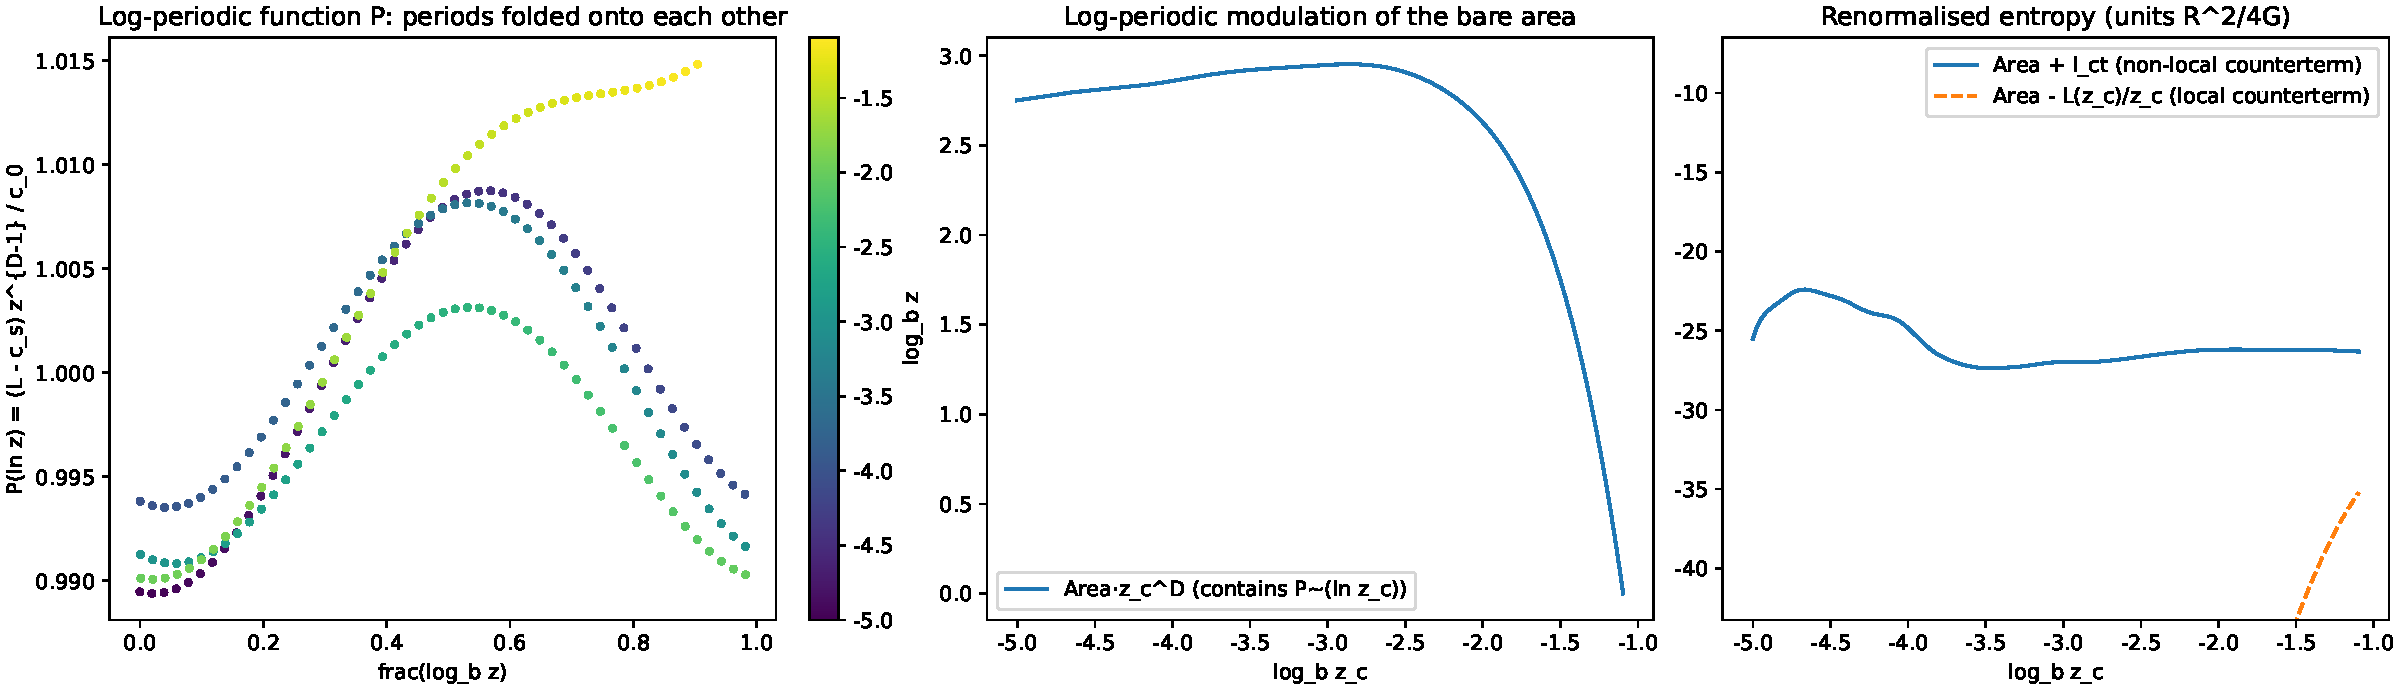
\includegraphics[width=\textwidth]{rt_renormalization}
\caption{Left: log-periodic function $P$ folded over periods. Middle: bare area times $z_c^{D}$. Right:
renormalised entropy with the non-local counterterm~\eqref{eq:Ict} (solid) and with the local counterterm
(dashed).}
\label{fig:ren}
\end{figure}

%=====================================================================
\section{Marginal complex dimensions}
\label{sec:marginal}

Poles with $\mathrm{Re}\,\omega>0$ produce power divergences, which Proposition~\ref{prop:ct} removes. Poles on
the line $\mathrm{Re}\,\omega=0$ are \emph{marginal}. A real pole at $\omega=0$ gives a logarithm, as for
corners~\cite{HirataTakayanagi,MyersSingh,BMWK}, and non-real poles $\omega=it$ give terms
$\varepsilon^{-it}/(it)$ that neither diverge nor decay. Such terms survive any minimal subtraction. In this
section we determine when they occur.

\subsection{Thread landing and the distance zeta function}
To analyse marginal terms we need more than the content $\cA(z)$: we need to know where on the boundary the
entanglement measured at depth $z$ resides. Bit threads (Section~\ref{sec:threads}) provide this. For a
half-space $A=\{x<0\}$, the geodesic flow of Proposition~\ref{prop:threads} consists of semicircles of radius
$u$ crossing $\gamma_A=\{x=0\}$ at depth $z=u$ and landing at distance $u$ from $\partial A$. Equating the flux
through $\gamma_A\cap\{u<z<u+\dd u\}$ with the number of threads landing in the corresponding boundary
strip shows that the landing density on $A$ is exactly
\begin{equation}
\varrho(y)=\frac{R^{d-1}}{4\GN}\,{\rm dist}(y,\partial A)^{-(d-1)} .
\label{eq:landing}
\end{equation}
For a general region we adopt~\eqref{eq:landing} as the leading near-boundary approximation, justified when
$\partial A$ is approximately planar on the scale ${\rm dist}(y,\partial A)$. This is the situation at depth
$z$ by Proposition~\ref{prop:kernel}, since there $\partial A$ is resolved only down to scale $z$. Then
\begin{equation}
S_A(\varepsilon)\simeq\frac{R^{d-1}}{4\GN}\int_{A,\ {\rm dist}>\varepsilon}{\rm dist}(y,\partial A)^{-(d-1)}\,\dd^{d-1}y
=\frac{R^{d-1}}{4\GN}\int_\varepsilon^{\delta}u^{-(d-1)}\,\dd V_A(u)+O(1),
\label{eq:distapprox}
\end{equation}
where $V_A(u)=|\{y\in A:{\rm dist}(y,\partial A)<u\}|$ is the inner tube volume. For smooth $\partial A$,
$V_A(u)=\Area(\partial A)\,u+O(u^2)$, which reproduces the area-law coefficient exactly.

Equation~\eqref{eq:distapprox} identifies the holographic entropy with the \emph{relative distance zeta
function} of Lapidus, Radunovi\'c and \v{Z}ubrini\'c~\cite{LRZ},
\begin{equation}
\zeta_{\partial A,A}(s)=\int_{A,\ {\rm dist}<\delta}{\rm dist}(y,\partial A)^{\,s-(d-1)}\,\dd^{d-1}y ,
\end{equation}
evaluated at $s=0$ and regulated at ${\rm dist}=\varepsilon$. Its poles are the complex dimensions of the
relative fractal drum $(\partial A,A)$. A pole $\omega$ with residue $c_\omega$ contributes
$c_\omega\varepsilon^{-\omega}/\omega$ to~\eqref{eq:distapprox} for $\omega\ne0$, and $c_0\ln(1/\varepsilon)$
for $\omega=0$. This is the precise sense in which the regulated value of the distance zeta function at $s=0$
is the AdS boundary contact term: the RT integrand $u^{-(d-1)}\dd V_A$ is exactly the distance-zeta
integrand at $s=0$. The tube formulas of Lapidus and collaborators~\cite{LvF,LRZ,LapidusPearse} expand $V_A$
as a sum over the same poles, so the divergence structure of $S_A$ is read off from the tube formula of
$\partial A$. Equation~\eqref{eq:distapprox} is an approximation. Corrections of the type $g(z)$ in
Theorem~\ref{thm:dsi} modify residues but, by that theorem, not pole locations on the critical line.

\subsection{The criterion}
For self-similar sprays and tilings the distance zeta function factorises~\cite{LRZ,LapidusPearse}:
\begin{equation}
\zeta_{\partial A,A}(s)=\frac{\zeta_{\rm gen}(s)}{M(s)}+(\text{entire}),\qquad
M(s)=1-\sum_jm_j\,r_j^{\,s}.
\label{eq:factor}
\end{equation}
Here $\zeta_{\rm gen}$ is the distance zeta function of the generator and $m_j$ counts copies with ratio $r_j$.
In the lattice case, $r_j=b^{-k_j}$ with $\gcd(k_j)=1$, set $x=b^{-s}$ and define the \emph{Moran polynomial}
\begin{equation}
\mathcal P(x)=\sum_jm_jx^{k_j}-1,\qquad M(s)=-\mathcal P(b^{-s}).
\end{equation}

\begin{theorem}[Marginal criterion]
\label{thm:marginal}
Assume~\eqref{eq:distapprox} and~\eqref{eq:factor}. The holographic entropy contains a bounded, non-decaying
log-periodic term, i.e.\ $\zeta_{\partial A,A}$ has a non-real pole on $\mathrm{Re}\,s=0$, if and only if
at least one of the following holds:
\begin{enumerate}
\item[(i)] $\mathcal P$ has a root $x_*=e^{-i\theta}$ on the unit circle, $\theta\notin2\pi\ZZ$, and
$\zeta_{\rm gen}(i\theta/\ln b)\ne0$ (counting the order of a possible zero of $\zeta_{\rm gen}$ against
the multiplicity of the root);
\item[(ii)] $\zeta_{\rm gen}$ has a non-real pole on $i\RR$ that is not cancelled by a zero of $1/M$.
\end{enumerate}
\end{theorem}
\begin{proof}
Poles of the quotient~\eqref{eq:factor} on $i\RR$ are either zeros of $M$ not cancelled by zeros of the
numerator, or poles of $\zeta_{\rm gen}$ not cancelled by poles of $M$. Since $M$ is entire, it has no poles,
so the second case is exactly (ii). For the first, $M(it)=0$ iff $\mathcal P(e^{-it\ln b})=0$, i.e.\ iff
$\mathcal P$ has a root on the unit circle. The root $x=1$ is excluded because
$\mathcal P(1)=\sum_jm_j-1\ge1$ for a genuine fractal ($\sum m_j\ge2$). By~\eqref{eq:distapprox} a simple
pole $\omega=it$ with residue $c_\omega$ contributes $c_\omega\varepsilon^{-it}/(it)$, which is bounded and does
not decay. A pole at $s=0$ itself contributes $\ln(1/\varepsilon)$ instead.
\end{proof}

\begin{corollary}[Single-ratio fractals]
\label{cor:koch}
If all ratios are equal, $r_j=1/b$ with $N$ copies, then $\mathcal P(x)=Nx-1$ has its only root at $1/N$,
inside the unit disk, so (i) never holds. In particular, for the Koch curve ($N=4$, $b=3$), whose generator is
polygonal and has only real poles, the marginal line carries only the real pole $s=0$. The entropy then
contains a universal logarithm,
\begin{equation}
S_A\supset\lambda\,\frac{R^{d-1}}{4\GN}\ln\frac1\varepsilon,\qquad
\lambda=\frac{\mathrm{Res}_{s=0}\zeta_{\rm gen}}{M(0)}=\frac{\mathrm{Res}_{s=0}\zeta_{\rm gen}}{1-N},
\end{equation}
but no bounded oscillation. The residue at $s=0$ of a polygonal generator comes from its corners, so this
is a renormalised corner logarithm~\cite{HirataTakayanagi}: the corners of all generations are resummed by the
factor $1/(1-N)$.
\end{corollary}

\subsection{An explicit lattice example}
Consider the lattice string with one copy of ratio $2^{-1}$ and one of ratio $2^{-5}$. Its Moran polynomial
factorises as
\begin{equation}
\mathcal P(x)=x^5+x-1=(x^2-x+1)(x^3+x^2-1).
\end{equation}
To verify, expand the right-hand side:
$x^5+x^4-x^2-x^4-x^3+x+x^3+x^2-1=x^5+x-1$.

The first factor is the cyclotomic polynomial $\Phi_6$, with roots $x=e^{\pm i\pi/3}$ on the unit circle.
The cubic has one real root $x_0\simeq0.7549$, giving $D=\ln(1/x_0)/\ln2\simeq0.4057$. Its other two roots
have modulus $x_0^{-1/2}\simeq1.151$, giving $\mathrm{Re}\,s\simeq-0.2028$. The complex dimensions are therefore
\begin{equation}
s\in\Big\{D+\tfrac{2\pi i m}{\ln2}\Big\}\cup\Big\{\tfrac{2\pi i}{\ln2}\big(m\pm\tfrac16\big)\Big\}
\cup\Big\{-0.2028+\dots\Big\},\qquad m\in\ZZ .
\end{equation}
The marginal family produces a bounded oscillation whose fundamental period in $\ln\varepsilon$ is $6\ln2$.

The mechanism is combinatorial. Let $c_K$ be the number of copies at log-depth $K$, i.e.\ with ratio
$2^{-K}$. It obeys $c_K=c_{K-1}+c_{K-5}$, whose generating function is $-1/\mathcal P(x)$. The factor $\Phi_6$
gives $c_K$ an exactly periodic, undamped component of period $6$ in $K$, on top of the growing component
$x_0^{-K}$. The growing component, weighted by $r^{\,D}$, produces the power divergence. The periodic component
enters the marginal (scale-invariant, $r^0$-weighted) term, where it cannot be removed by any counterterm
targeting $\mathrm{Re}\,\omega>0$. More generally, a cyclotomic factor $\Phi_n$ of $\mathcal P$ gives a period
$n\ln b$. Unit-circle roots that are not roots of unity would give quasi-periodic marginal terms; we have not
classified when they occur.

\paragraph{Numerical check.} In an exactly solvable renewal model with generator $g(u)=ue^{-u}$, so that
$\zeta_g=\Gamma(s)$ has only real poles, we computed $S(\varepsilon)=\int_\varepsilon^1z^{-2}\cA\,\dd z$ exactly and
subtracted all poles with $\mathrm{Re}\,\omega>0$ and the logarithm $\ln(1/\varepsilon)/M(0)$. For the Koch-type
system the remainder is constant to $9\times10^{-4}$. For the $(2^{-1},2^{-5})$ string it oscillates with
peak-to-peak amplitude $0.16$ and period $6\ln2$, agreeing with the Mellin prediction
$\sum_{\mathrm{Re}\,\omega=0}c_\omega\varepsilon^{-\omega}/\omega$ to $3\times10^{-4}$ (Fig.~\ref{fig:dsi}).

\begin{figure}[htbp]
\centering
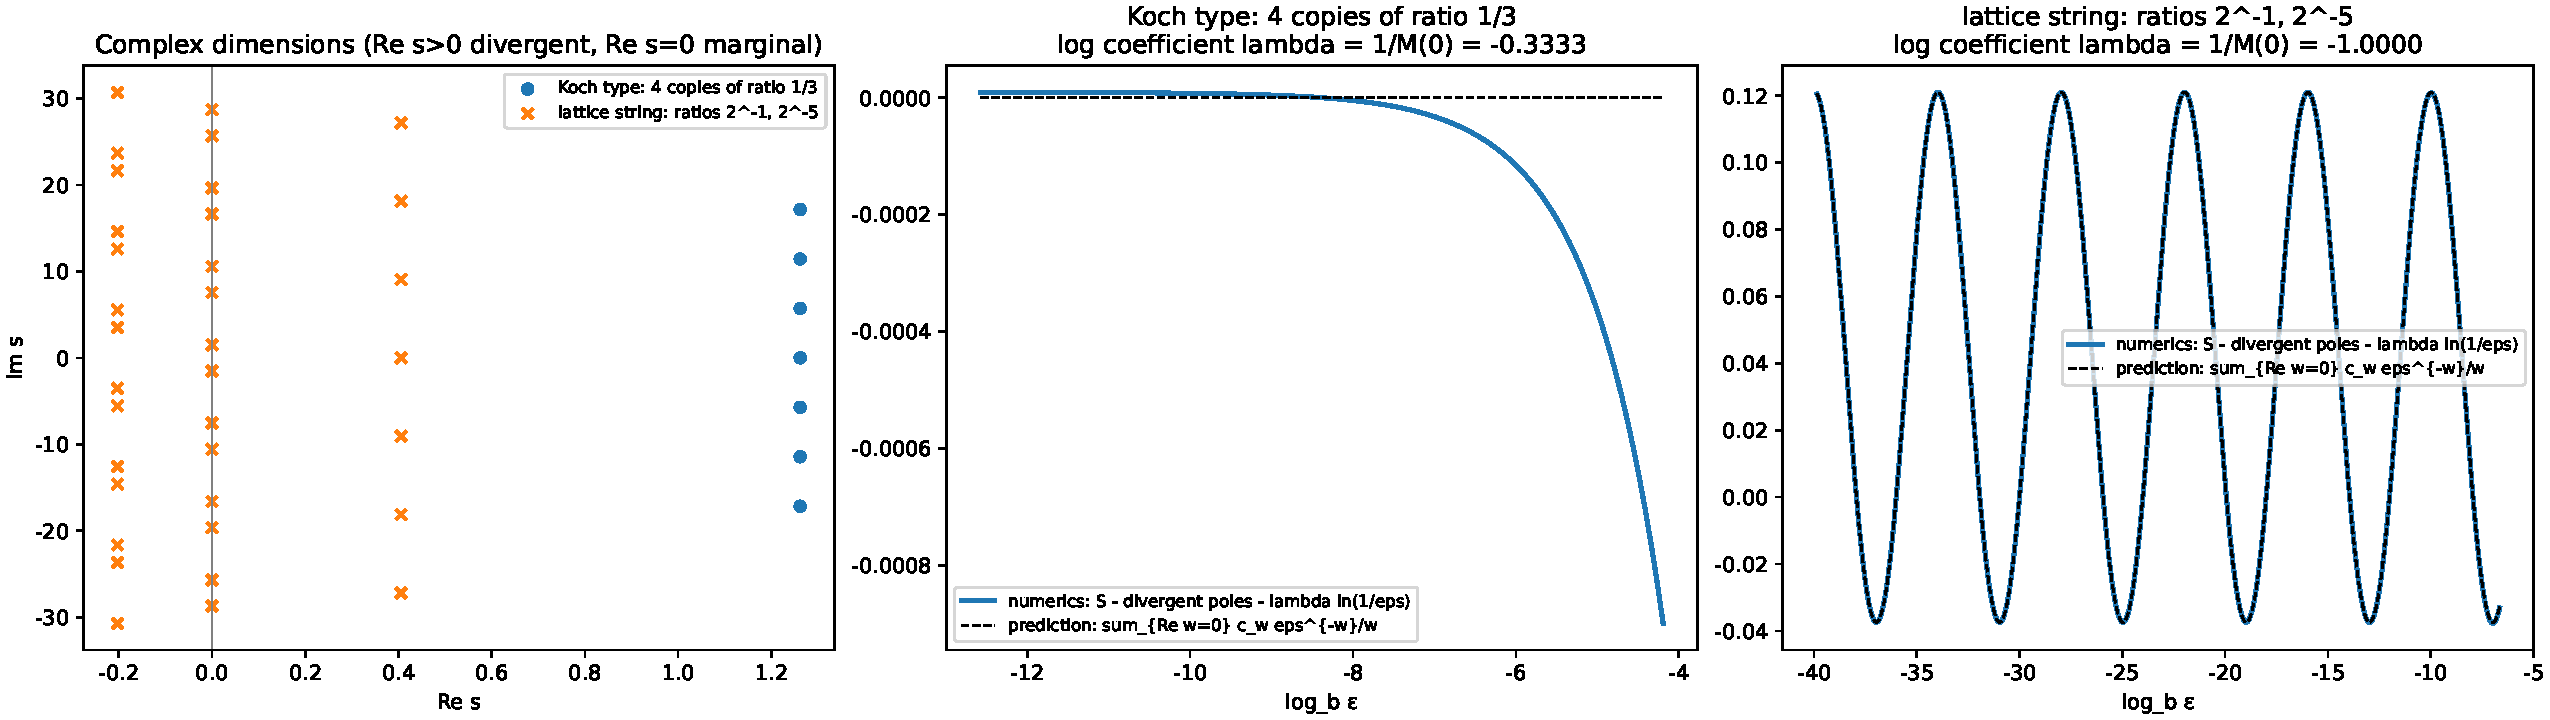
\includegraphics[width=\textwidth]{dsi_complex_dims}
\caption{Left: complex dimensions of the Koch-type system and the $(2^{-1},2^{-5})$ lattice string. Middle
and right: renormalised entropy after subtracting divergent poles and the logarithm (solid) against the
prediction from marginal complex dimensions (dashed).}
\label{fig:dsi}
\end{figure}

%=====================================================================
\section{R\'enyi entropies, cosmic branes and multifractality}
\label{sec:renyi}

\subsection{Dong's area law and its thermodynamic reading}
For a holographic CFT, Dong showed that~\cite{Dong}
\begin{equation}
\tilde S_q\equiv q^2\partial_q\Big(\frac{q-1}{q}S_q\Big)=\frac{\Area(\mathcal C_q)}{4\GN},
\label{eq:dong}
\end{equation}
where $\mathcal C_q$ is a cosmic brane with tension $T_q=(q-1)/(4q\GN)$. The brane backreacts on the bulk by
creating a conical deficit $\Delta\phi=2\pi(q-1)/q$, and the replica derivation follows Lewkowycz and
Maldacena~\cite{LM}. Dong also noted that $\tilde S_q=-\partial F_q/\partial T$ with
$F_q=-\frac1q\ln\mathrm{Tr}\rho^q$ and $T=1/q$. In other words, $\tilde S_q$ is the thermodynamic entropy of
the modular Hamiltonian $K=-\ln\rho$ at temperature $1/q$, i.e.\ the von Neumann entropy of the escort state
$\rho_q=\rho^q/\mathrm{Tr}\rho^q$. He cited the thermodynamic formalism of Beck and
Schl\"ogl~\cite{BeckSchlogl} and Baez~\cite{Baez}; see also~\cite{NakaguchiNishioka}.

\subsection{Cosmic-brane areas as a singularity spectrum}
The thermodynamic formalism of multifractals~\cite{Halsey,BeckSchlogl} applies verbatim once
$\mathrm{Tr}\rho_A^q$ scales with the cutoff. We record the resulting identity.

\begin{proposition}[Brane area and singularity spectrum]
\label{prop:brane}
Let $\mathcal L\to\infty$ be a large parameter, for instance $\mathcal L=\ln(1/\varepsilon)$, and suppose
\begin{equation}
\ln\mathrm{Tr}\rho_A^q=-\tau(q)\,\mathcal L+o(\mathcal L)
\label{eq:tau}
\end{equation}
pointwise on an open interval $I$ of $q$ on which $\tau$ is differentiable. Then for every $q\in I$,
\begin{equation}
\frac{\tilde S_q}{\mathcal L}\to f(\alpha_q)\equiv q\alpha_q-\tau(q),\qquad
\frac{\langle K\rangle_{\rho_q}}{\mathcal L}\to\alpha_q\equiv\tau'(q),
\label{eq:fbrane}
\end{equation}
so that, by~\eqref{eq:dong}, $\Area(\mathcal C_q)/4\GN=f(\alpha_q)\,\mathcal L\,(1+o(1))$.
\end{proposition}
\begin{proof}
$\Phi(q):=\ln\mathrm{Tr}\rho^q$ is convex in $q$, since it is a log-sum-exp of functions linear in $q$.
Pointwise convergence of the differentiable convex functions $\Phi/\mathcal L\to-\tau$ on $I$, with
differentiable limit, implies convergence of their derivatives on $I$~\cite[Thm.~25.7]{Rockafellar}, so
$-\Phi'/\mathcal L\to\tau'$. Since $\frac{q-1}{q}S_q=-\frac1q\Phi$, we get
$\tilde S_q=q^2\partial_q(-\Phi/q)=\Phi-q\Phi'$, hence $\tilde S_q/\mathcal L\to-\tau+q\tau'$. Finally
$\langle K\rangle_{\rho_q}=-\Phi'(q)$.
\end{proof}
The proof is two lines, and we claim no novelty for the identity: it is the standard Legendre structure of
the thermodynamic formalism transcribed through~\eqref{eq:dong}. Its use here is interpretive. The tension of
the brane selects a Hölder exponent $\alpha_q$, and the brane area counts the eigenvalues of $\rho_A$ near
$e^{-\alpha_q\mathcal L}$. The multifractal spectrum of the entanglement spectrum is therefore a
\emph{geometric} quantity in the bulk, namely the area of a one-parameter family of cosmic branes.

\subsection{Einstein gravity: the shape of $f$ is fixed by the bulk}
For a spherical (or planar) entangling surface the backreacted geometry is a hyperbolic black
hole~\cite{HMSY,Dong}:
\begin{equation}
\dd s^2=f(r)\dd\tau^2+\frac{\dd r^2}{f(r)}+r^2\dd H_{d-1}^2,\qquad f(r)=r^2-1-\frac{r_h^{d}-r_h^{d-2}}{r^{d-2}}\quad(R=1).
\end{equation}
Its temperature is $T(r_h)=f'(r_h)/4\pi=(dr_h^2-(d-2))/(4\pi r_h)$, with $T(1)=T_0=1/2\pi$. Smoothness of the
$q$-fold cover, equivalently the deficit $2\pi(q-1)/q$ in the quotient, requires $T(x_q)=T_0/q$:
\begin{equation}
dx_q^2-\frac{2}{q}x_q-(d-2)=0\quad\Longrightarrow\quad x_q=\frac{1+\sqrt{1+d(d-2)q^2}}{dq}.
\end{equation}
The brane sits at the horizon, so $\tilde S_q=x_q^{d-1}S_1$, and~\cite{HMSY}
\begin{equation}
\frac{S_q}{S_1}=\frac{q}{2(q-1)}\Big(2-x_q^{d-2}(1+x_q^2)\Big).
\end{equation}
With $\mathcal L=S_1$, Proposition~\ref{prop:brane} gives $f(\alpha_q)=x_q^{d-1}$ and
$\alpha_q=\partial_q[(q-1)S_q/S_1]$. We verified $q^2\partial_q(\frac{q-1}{q}S_q)/S_1=x_q^{d-1}$ numerically to
$10^{-8}$ for $d=2,3,4$.

For a fractal entangling surface the near-boundary part of the brane at depth $z$ sees a locally planar
surface (Proposition~\ref{prop:kernel}). To leading order the R\'enyi entropies then factorise:
\begin{equation}
S_q^{\rm div}\simeq\Big(\frac{S_q}{S_1}\Big)_{\rm grav}\times S_1^{\rm div},\qquad
S_1^{\rm div}\propto N_\varepsilon(\partial A).
\end{equation}
The geometry of $\partial A$ fixes only the overall scale $\mathcal L$; the shape of $f(\alpha)$ is fixed by the
gravitational theory. This factorisation is an approximation that we have not proven for fractal surfaces.

\paragraph{The case $d=2$.} Here $x_q=1/q$. Writing $\mathcal L=\ln(\ell/\varepsilon)$ for an interval,
\begin{equation}
\tau(q)=\frac c6\Big(q-\frac1q\Big),\quad \alpha_q=\frac c6\Big(1+\frac1{q^2}\Big),\quad
f(\alpha_q)=\frac{c}{3q},\qquad
f(\alpha)=\sqrt{\frac c3\Big(2\alpha-\frac c3\Big)},\ \ \alpha\ge\frac c6 .
\label{eq:CLf}
\end{equation}
This is the exponential growth rate of the Calabrese--Lefevre eigenvalue density~\cite{CL}. It can be
recovered from the BCFT description of Cardy and Tonni~\cite{CT}, as follows. The reduced density matrix is
the annulus of width $W=2\mathcal L$, whose open-channel eigenvalues are
\begin{equation}
\lambda_h=\frac{e^{-(2\pi^2/W)(h-c/24)}}{Z(W)},
\label{eq:CTweights}
\end{equation}
with $h$ the dimensions of boundary-condition-changing operators. The closed channel gives
$\ln Z=cW/12+O(1)$. With the Cardy density $\rho(E)\sim e^{2\pi\sqrt{cE/6}}$, $E=h-c/24$, the eigenvalues at
$\alpha=-\ln\lambda/\mathcal L$ have $E=\mathcal L^2(\alpha-c/6)/\pi^2$, and their number is
$e^{2\pi\sqrt{cE/6}}=e^{\mathcal L\sqrt{(2c/3)(\alpha-c/6)}}$, which is~\eqref{eq:CLf}. We present this as a
consistency check between~\eqref{eq:dong}, \cite{CT} and~\cite{CL}, not as a new result. Numerically, the
saddle-point prediction is approached with deviation $8\times10^{-2}$ ($W=400$) and $2.4\times10^{-2}$
($W=2000$), in units of $c/6$ (Fig.~\ref{fig:bcft}).

\subsection{Sparse spectra and the $1/c$ tension}
Equation~\eqref{eq:CTweights} gives Schmidt weights of the form $p\propto e^{-\alpha\Delta}$ with
$\alpha=2\pi^2/W$. Suppose, as a model assumption, that for a self-similar region the modular Hamiltonian
factorises across generations, each generation $j$ being an annulus of log-width $\lambda_j=\ln(1/r_j)$.
The cascade weights are then
\begin{equation}
p_j\propto n_j\,e^{-(2\pi^2/\lambda_j)\Delta_j},\qquad \sum_jp_j^{\,q}\,r_j^{-\tau(q)}=1 .
\end{equation}
For a dense (Cardy) spectrum the shape of $f$ is again universal. Non-trivial multifractality requires a
\emph{sparse} spectrum of $\Delta_j$. For Ising boundary-condition-changing operators,
$\Delta\in\{0,1/16,1/2\}$, with $b=3$ we find $p=(0.754,0.245,9\times10^{-5})$ and $D_1=0.51$.

This exposes a tension. Classical (large-$c$) holography implies Cardy-like density and hence a universal
shape of $f$ fixed by $x_q$. Sparse spectra, needed for non-trivial cascade weights, are not described by
Einstein gravity. In a holographic theory, cascade-type multifractality can therefore appear only at
$O(c^0)$: in bulk quantum corrections~\cite{FLM}, or in superpositions of fixed-area
states~\cite{DHM,AkersRath}. We have not derived $p_j$ from first principles beyond the factorised model.

Finally, for a lattice cascade the partition function obeys a renewal equation whose poles are at
$\tau(q)+2\pi im/\ln b$. The argument of Theorem~\ref{thm:dsi}, Step 3, with weights
$w_j(q)=p_j^qr_j^{-\tau(q)}>0$ summing to $1$, shows that the imaginary parts are $q$-independent. We
confirmed this numerically for $r=(1/2,1/4)$, where the oscillation has period $\ln2$ for $q=-2,0,2,4$. For
a non-lattice cascade the oscillation is not periodic (Fig.~\ref{fig:lockin}).

\begin{figure}[htbp]
\centering
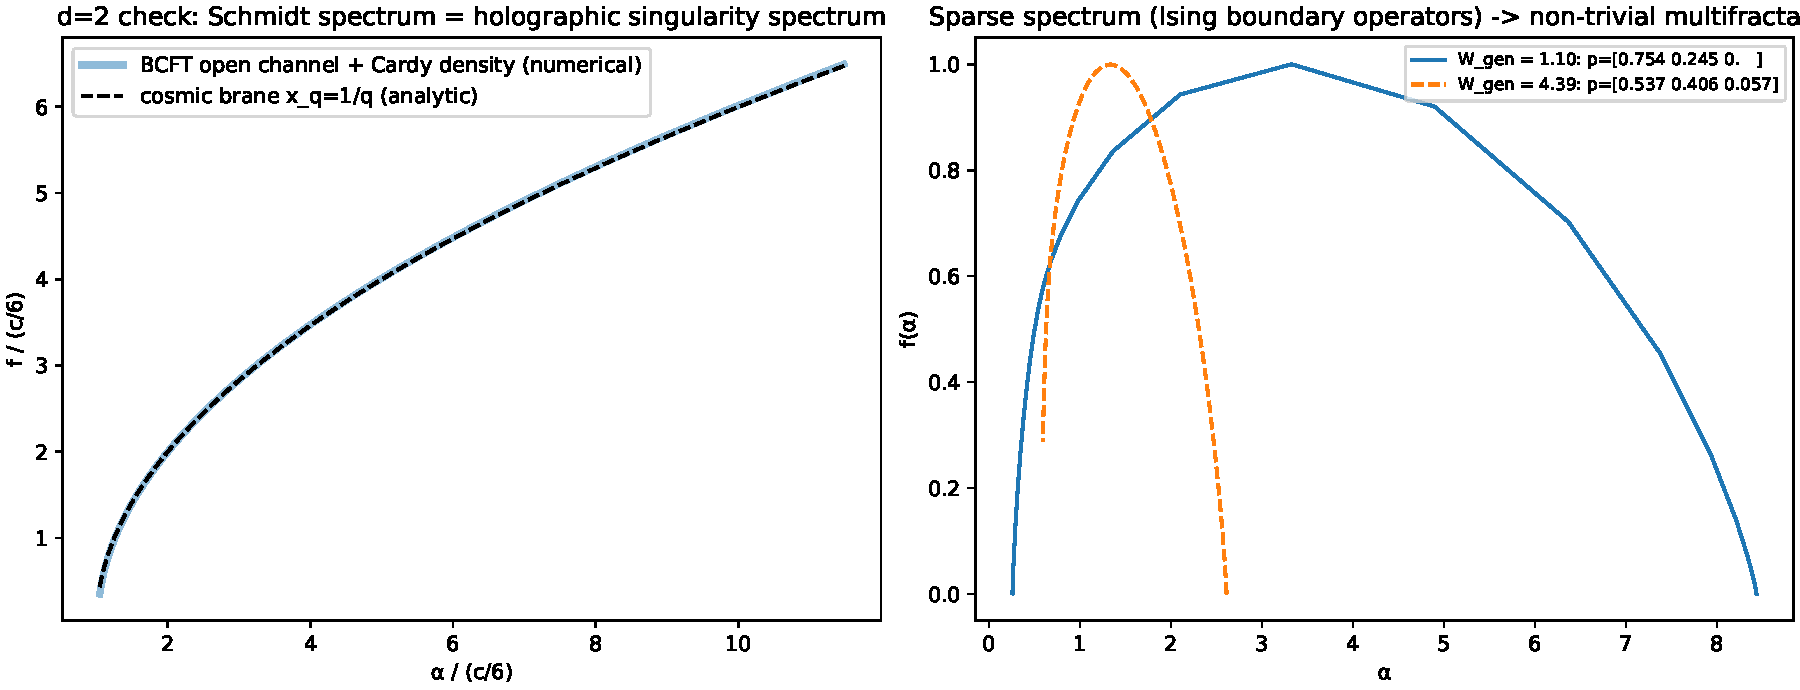
\includegraphics[width=0.9\textwidth]{bcft_closure}
\caption{Left: singularity spectrum from BCFT open-channel weights with Cardy density (numerical) against the
cosmic-brane result~\eqref{eq:CLf}. Right: cascade spectra from Ising boundary operators.}
\label{fig:bcft}
\end{figure}
\begin{figure}[htbp]
\centering
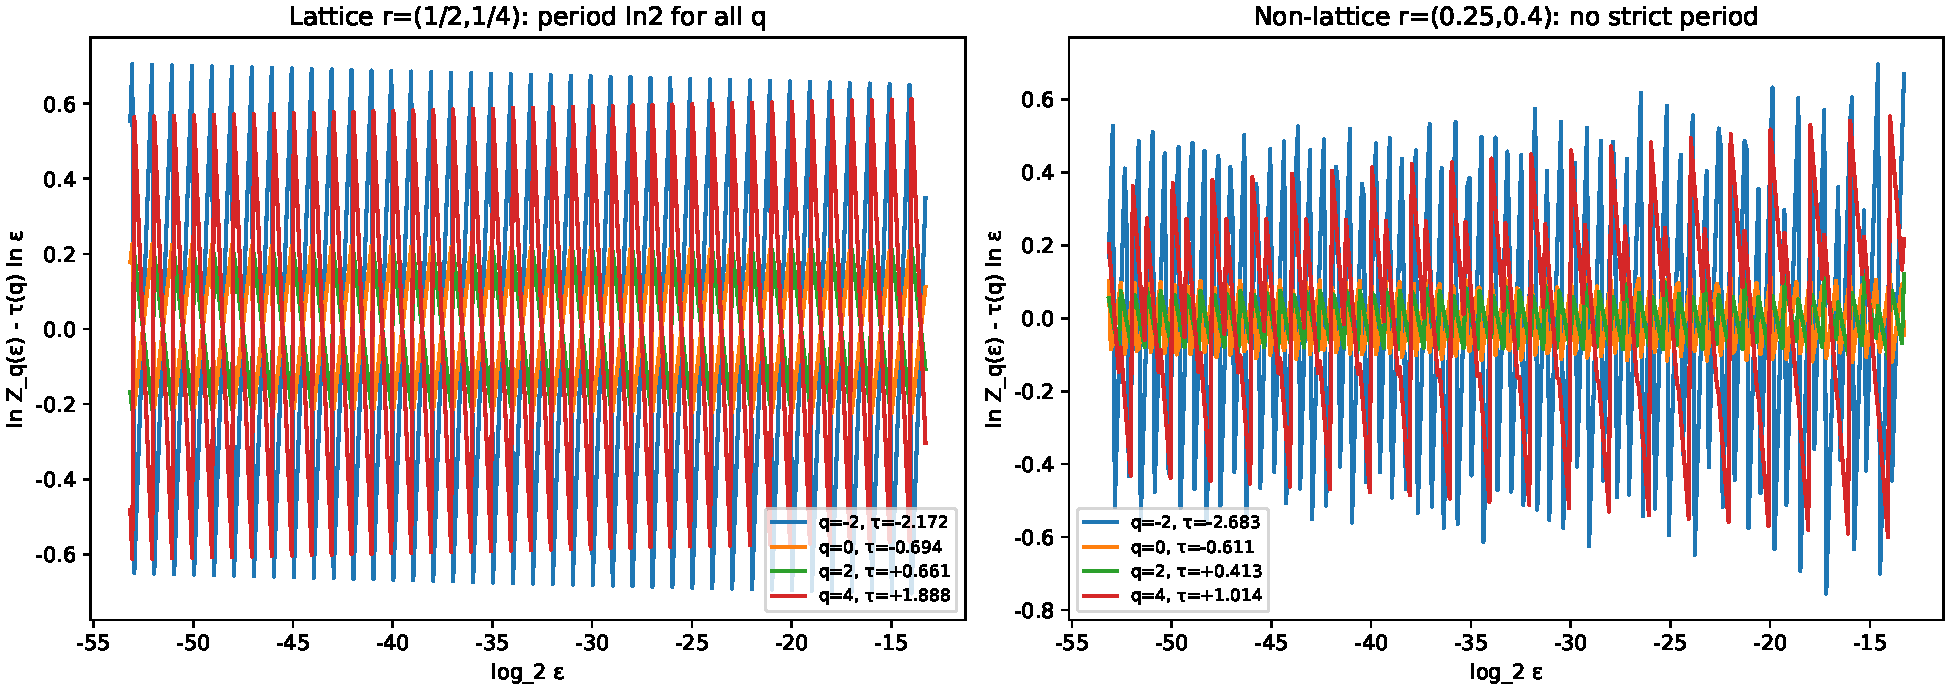
\includegraphics[width=0.9\textwidth]{multifractal_lockin}
\caption{$\ln Z_q(\varepsilon)-\tau(q)\ln\varepsilon$ for lattice (left) and non-lattice (right) binomial
cascades.}
\label{fig:lockin}
\end{figure}

%=====================================================================
\section{Bit threads and scale transport}
\label{sec:threads}

\subsection{Flux depth distribution and geodesic flows}
Freedman and Headrick showed that~\cite{FH}
\begin{equation}
S_A=\max_v\int_Av,\qquad \nabla_\mu v^\mu=0,\qquad |v|\le\frac1{4\GN},
\end{equation}
and that every maximal flow saturates the bound normal to $\gamma_A$. Explicit flows were constructed
in~\cite{ABP}. We adapt their geodesic construction to the planar case.

\begin{proposition}[Thread depth distribution and geodesic flow]
\label{prop:threads}
\begin{enumerate}
\item[(i)] The flux through $\gamma_A\cap\{z_1<z<z_2\}$ is the same for every maximal flow and equals
$\int_{z_1}^{z_2}n(z)\dd z$, with
\begin{equation}
n(z)=\frac{R^{d-1}}{4\GN}z^{1-d}\cA(z)=\frac{R}{4\GN}\frac{V(z)}{z},
\end{equation}
independent of the flow.
\item[(ii)] The flux lost when the cutoff is raised, $-\partial_{z_c}\Phi(z_c)=n(z_c)$, is related to the
counterterm~\eqref{eq:Ict} by $\partial_{z_c}I_{ct}=\Pi_+n(z_c)$.
\item[(iii)] For a half-space $A=\{x<0\}$, the vector field tangent to the semicircles $x^2+z^2=u^2$ (at fixed
$\vec y$), with
\begin{equation}
|v|=\frac{\sin^{d-1}\theta}{4\GN},\qquad \sin\theta=\frac zu,
\label{eq:geoflow}
\end{equation}
is divergence-free and satisfies $|v|\le1/4\GN$, with equality exactly on $\gamma_A=\{x=0\}$.
\end{enumerate}
\end{proposition}
\begin{proof}
(i) On $\gamma_A$ a maximal flow has $v\cdot n=1/4\GN$~\cite{FH}, so the flux through a portion of $\gamma_A$
is its area divided by $4\GN$. The area element is given by Lemma~\ref{lem:radial}.
(ii) The first statement follows from (i). The second is~\eqref{eq:flow} rewritten using
$n=(R/4\GN)V/z$.

(iii) On the slice~\eqref{eq:slice}, $g_{\mu\nu}=(R^2/z^2)\delta_{\mu\nu}$ and $\sqrt g=(R/z)^d$, so
\begin{equation}
\nabla_\mu v^\mu=\frac{1}{\sqrt g}\,\partial_\mu\big(\sqrt g\,v^\mu\big).
\end{equation}
Semicircles orthogonal to the boundary are geodesics of $\mathbb H^d$. In the $(x,z)$ plane the coordinate
unit tangent, oriented from $A$ to $\bar A$, is $t=(z,-x)/u$. The corresponding proper unit vector is
$\hat v=(z/R)\,t$, because $|t|_g=(R/z)|t|_\delta$. With $v=\frac1{4\GN}(z/u)^{d-1}\hat v$, the only
non-zero components are
\begin{equation}
\sqrt g\,v^x=\frac{R^{d-1}}{4\GN}\frac{z}{u^d},\qquad \sqrt g\,v^z=-\frac{R^{d-1}}{4\GN}\frac{x}{u^d},
\qquad u=\sqrt{x^2+z^2}.
\end{equation}
Hence
\begin{equation}
\partial_x\Big(\frac{z}{u^d}\Big)-\partial_z\Big(\frac{x}{u^d}\Big)
=-\frac{d\,xz}{u^{d+2}}+\frac{d\,xz}{u^{d+2}}=0,
\end{equation}
and $\nabla_\mu v^\mu=0$; the $\vec y$-components vanish identically. The norm is
$|v|=\frac1{4\GN}(z/u)^{d-1}\le\frac1{4\GN}$, with equality iff $z=u$, i.e.\ $x=0$. There $\hat v=\partial_x$
in proper normalisation, so $v\cdot n=1/4\GN$ and the bound is saturated on $\gamma_A$. (The computation was
also checked symbolically.)
\end{proof}
Part (iii) is the planar limit of the construction of~\cite{ABP}. Parts (i)--(ii) give the counterterm a
direct interpretation: $I_{ct}$ removes exactly the threads whose depth distribution lies in the divergent
complex-dimension modes, and $S_{\rm ren}=\lim_{z_c\to0}\int_{z_c}(1-\Pi_+)n\,\dd z$.

\paragraph{R\'enyi threads (proposal).} Since $\tilde S_q$ is the area of $\mathcal C_q$ in the backreacted
geometry $g_q$, max-flow/min-cut on the time slice of $g_q$ gives $\tilde S_q=\max\int_Av_q$, \emph{provided}
$\mathcal C_q$ is minimal, not merely extremal, on that slice. Under this assumption the loss rate of
$q$-threads per $e$-fold of $z$ is $f(\alpha_q)\,\partial_\ell\mathcal L$ with $\ell=\ln(1/z)$, by
Proposition~\ref{prop:brane}. We have not established the minimality assumption in general.

\subsection{A scale-transport equation}
The preceding results share one structure: a quantity at log-scale $\ell=\ln(\ell_0/z)$ is a weighted sum of
copies of itself at shifted scales, plus a source. We propose this structure as an organising principle.

\begin{conjecture}[Scale transport]
\label{conj:transport}
For a self-similar $\partial A$ with similarities $S_j$, $\lambda_j=\ln(1/r_j)$, there exist state-dependent
weights $p_j>0$, $\sum_jp_j=1$, and a source $\sigma_\ell$ of lower growth, such that the measure $\rho_\ell$
describing the entanglement (thread landing) density resolved at scale $\ell$ satisfies
\begin{equation}
\rho_\ell=\sum_jp_j\,(S_j)_\sharp\,\rho_{\ell-\lambda_j}+\sigma_\ell .
\label{eq:transport}
\end{equation}
Here $(S_j)_\sharp$ is the push-forward, so the right side is the Hutchinson operator~\cite{Hutchinson}
acting along a renewal in $\ell$.
\end{conjecture}

Taking $q$-th moments over a partition at resolution $e^{-\ell}$ gives
$Z_q(\ell)=\sum_jp_j^{\,q}Z_q(\ell-\lambda_j)+G_q(\ell)$. Its Laplace transform has poles at the complex mass
exponents $\tau(q)+i\Lambda^\perp$. If Conjecture~\ref{conj:transport} holds, the results of this paper are
its specialisations:
\begin{center}
\begin{tabular}{ll}
\toprule
Specialisation & Result\\
\midrule
geometric weights $p_j=r_j^{D_\partial}$ ($q=0$ data) & complex dimensions, Theorem~\ref{thm:dsi}\\
poles with $\mathrm{Re}>0$ & non-local counterterm, Proposition~\ref{prop:ct}\\
poles on $\mathrm{Re}=0$ & logarithms and bounded oscillations, Theorem~\ref{thm:marginal}\\
Legendre transform in $q$ & cosmic-brane areas, Proposition~\ref{prop:brane}\\
$-\partial_\ell$ of the first moment & thread loss rate, Proposition~\ref{prop:threads}\\
\bottomrule
\end{tabular}
\end{center}
The conjecture is established only in two cases. The first is the geometric case, where it reduces to the
renewal equation~\eqref{eq:renewal}, subject to Lemma~\ref{lem:decoupling}. The second is the factorised BCFT
model of the previous section, where it holds by assumption. We do not derive non-geometric weights $p_j$ from
first principles, and~\eqref{eq:transport} should be read as a framework rather than a theorem.

\section{Experimental fingerprint: lattice fractal-string resonators}
\label{sec:exp}
The renewal and zeta-function structure behind marginal complex dimensions is not specific to holography.
It governs the spectral asymptotics of fractal strings~\cite{LvF}, produces log-periodic terms in the
thermodynamics of fields on fractals~\cite{ADT}, and has been discussed as an observable signature of
discrete scale invariance~\cite{Calcagni}. This suggests a laboratory test of the structure that our
holographic analysis shares with fractal-string theory. We stress that such a test probes the
zeta-function mechanism of Section~\ref{sec:marginal}, not holography itself.

\paragraph{Geometry.} Consider a lattice fractal string generated by one copy of ratio $r_1=1/3$ and two
copies of ratio $r_2=1/9$, realised as a collection of one-dimensional resonators (for instance
transmission-line or acoustic resonators) of lengths $\ell_w=\ell_0r_w$, where $r_w$ is the product of the
ratios along the word $w$. Its geometric zeta function is $\zeta_L(s)=\sum_wr_w^{\,s}=1/M(s)$ with
\begin{equation}
M(s)=1-3^{-s}-2\cdot9^{-s}=-\mathcal P(3^{-s}),\qquad \mathcal P(x)=2x^2+x-1=(2x-1)(x+1).
\end{equation}
The root $x=1/2$ gives $D=\ln2/\ln3\simeq0.6309$. The root $x=-1$, a zero of the cyclotomic factor
$\Phi_2(x)=x+1$, places a marginal family exactly on the imaginary axis,
\begin{equation}
s_m^{(0)}=\frac{(2m+1)\pi i}{\ln3},\qquad m\in\ZZ ,
\end{equation}
and $\mathcal P$ has no other roots.

\paragraph{Observable.} With Dirichlet ends, the resonance frequencies are $f_{w,k}=kv/(2\ell_w)$,
$k\ge1$, where $v$ is the phase velocity. We use the heat-kernel-smoothed mode count
\begin{equation}
\Theta(u)=\sum_w\sum_{k\ge1}\exp\!\Big(-\frac{k^2}{(u\,r_w)^2}\Big),\qquad u=\frac{2\ell_0f}{v},
\end{equation}
which can be computed directly from a measured list of resonances. Its Mellin transform is
\begin{equation}
\int_0^\infty u^{-s-1}\Theta(u)\,\dd u=\tfrac12\,\Gamma(s/2)\,\zeta(s)\,\zeta_L(s),
\end{equation}
where $\zeta(s)$ is the Riemann zeta function, so that as $u\to\infty$
\begin{equation}
\begin{gathered}
\Theta(u)=\frac{\sqrt\pi}{2}\zeta_L(1)\,u+\sum_{m\in\ZZ}A_m^{(D)}u^{D+2\pi im/\ln3}+\frac14
+\sum_{m\in\ZZ}A_m^{(0)}u^{(2m+1)\pi i/\ln3}+\dots,\\
A=\frac{\Gamma(s/2)\zeta(s)}{2M'(s)}\Big|_{\rm pole}.
\end{gathered}
\label{eq:resonator}
\end{equation}
The constant is $\tfrac12\cdot2\cdot\zeta(0)/M(0)=1/4$. The poles of $\Gamma(s/2)$ at $s=-2,-4,\dots$ are
cancelled by the trivial zeros of $\zeta$, so the remainder decays faster than any power of $u$.

\paragraph{Fingerprint.} After the Weyl term is removed, a Fourier analysis in $\log_3u$ separates two
families of lines. The $D$ family gives \emph{integer} harmonics (an integer number of cycles per
$\log_3$ unit), with envelope growing as $u^D\propto f^D$. The marginal family gives \emph{half-integer}
harmonics with bounded, non-decaying amplitude. Numerically, the residual
$\Theta-\text{Weyl}-D\text{ family}-1/4$ agrees with the marginal sum in~\eqref{eq:resonator} to
$2\times10^{-6}$. Its peak-to-peak amplitude is $0.059$ modes, the fundamental has $|A_0^{(0)}|=0.0145$, and the
pattern repeats every factor $9$ in frequency (Fig.~\ref{fig:resonator}).

\paragraph{Requirements and caveats.} Two full periods of the marginal oscillation require a frequency ratio
of $81$. For example, with $\ell_0=10$\,cm and $v=1.2\times10^8$\,m/s the band is $0.60$--$48.6$\,GHz. Only
branches with $r_w\ge3^{-4}$ have modes in this band, and there are $1+1+3+5+11=21$ of them. The mean Weyl
spacing of resonances is $v/(2\ell_0\zeta_L(1))=\tfrac49\,v/(2\ell_0)\simeq0.27$\,GHz, independent of
frequency, so near the top of the band a quality factor of at least a few hundred is needed merely to
separate neighbouring resonances. Exact degeneracies between equal-length branches must be counted with
their multiplicity. Because the marginal amplitude is only $0.059$ modes, the count must be exact: a single
missed or spurious resonance in the analysed band is comparable to the signal. Fabrication tolerances on the
lengths shift resonances and must be included in an error budget, which we have not carried out. Finally,
for \emph{uncoupled} branches the spectrum is the union of harmonic ladders, and~\eqref{eq:resonator} follows
from the lengths alone. The experiment then tests the explicit formula and the realisability of the
measurement, not new physics. A physically non-trivial test would use a coupled network or a single
cavity with a lattice-self-similar boundary, for which the smoothed counting function is not additive. In
that case the pole \emph{locations} of~\eqref{eq:resonator} are still fixed by $M(s)$, but the residues are not.

\begin{figure}[htbp]
\centering
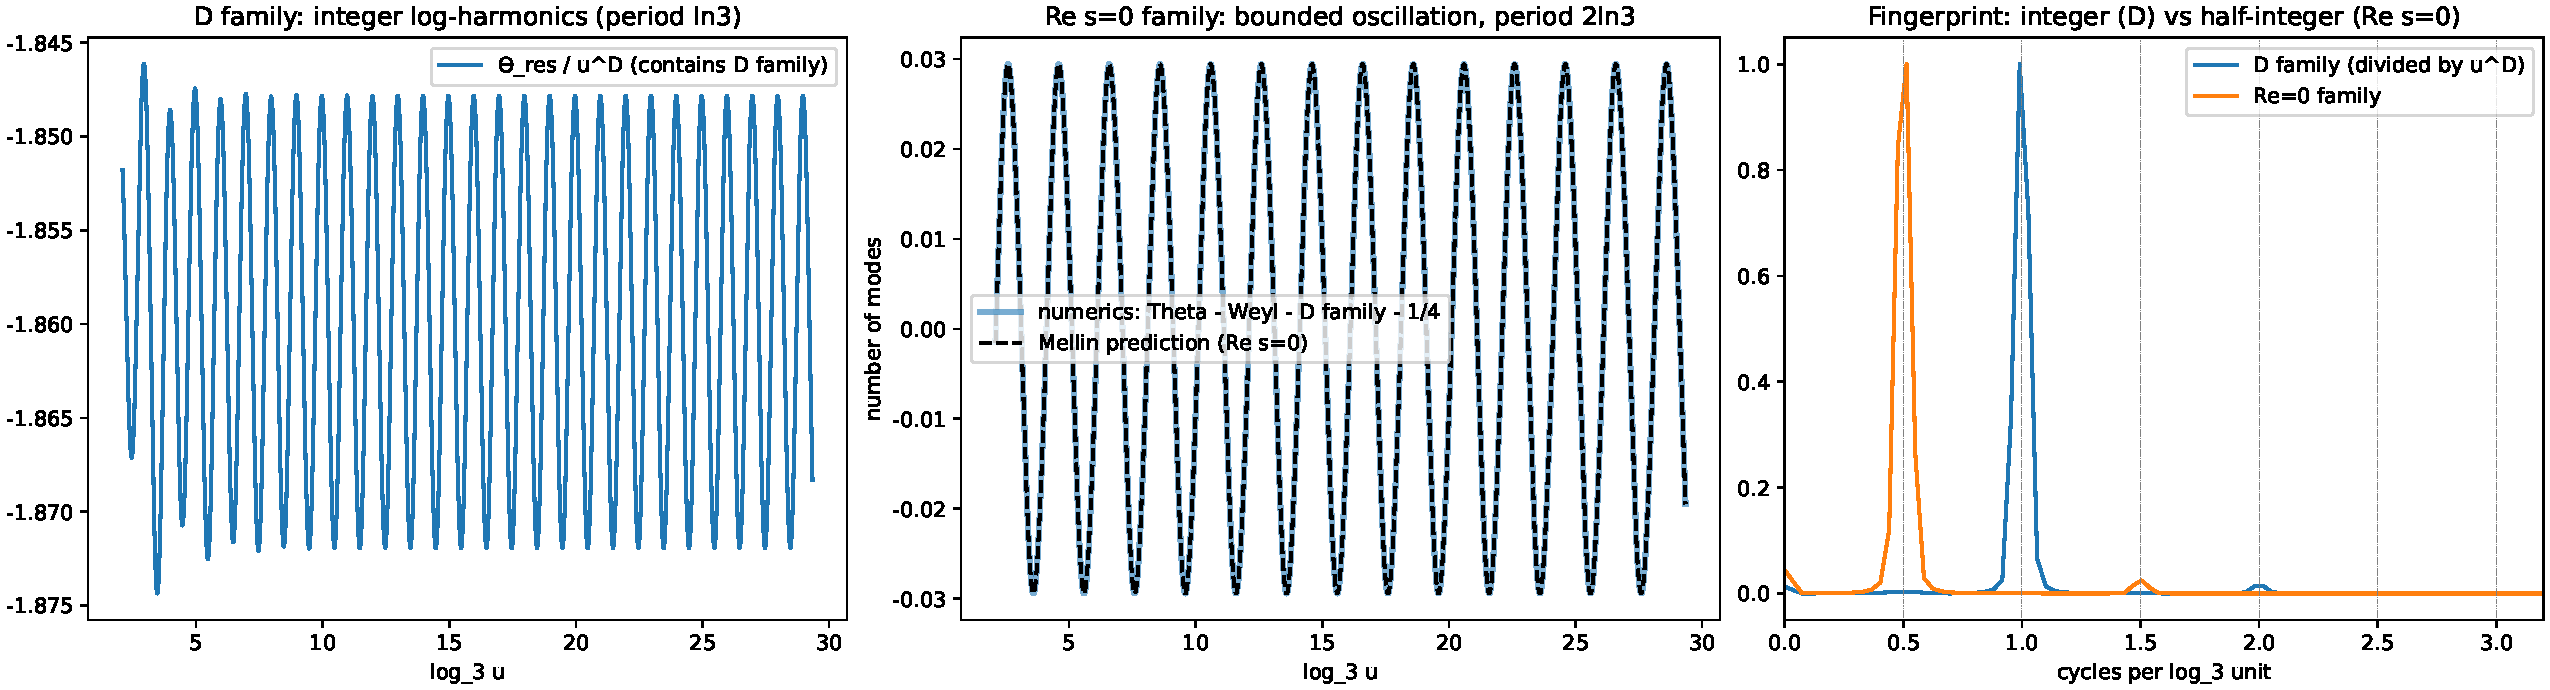
\includegraphics[width=\textwidth]{resonator_fingerprint}
\caption{Lattice fractal-string resonator. Left: residual heat trace divided by $u^D$, showing the integer
log-harmonics of the $D$ family. Middle: residual after removing the $D$ family, compared with the marginal
prediction from~\eqref{eq:resonator}. Right: Fourier spectra in $\log_3u$, with integer lines for the $D$
family and half-integer lines for the marginal family.}
\label{fig:resonator}
\end{figure}

\section{Discussion and limitations}
\label{sec:discussion}
We summarise what is established, what is assumed, and what remains open.
\begin{enumerate}
\item \emph{Near-boundary decoupling.} Lemma~\ref{lem:decoupling} is proven in the linearised RT problem,
with $\eta=d$, and is consistent with the Fefferman--Graham structure and with entanglement wedge
nesting~\cite{Wall}. Nesting, however, controls the deviation only qualitatively. A non-linear proof would
require quantitative barrier estimates for the minimal-surface equation in smooth AdS with non-rectifiable
(fractal) boundary data. Theorems~\ref{thm:dsi} and~\ref{thm:marginal} inherit this assumption.
\item \emph{Self-similar versus self-affine boundaries.} Theorem~\ref{thm:dsi} uses the fact that boundary
similarities extend to isometries of AdS. Anisotropic (self-affine) scalings do not, so self-affine
boundaries such as~\eqref{eq:weierstrass} are not covered beyond the linearised problem. In the linearised
model the effective exponent $D_{\rm fit}\neq D$ of Section~\ref{sec:table1} is due to mode truncation and to
the non-homogeneity of $\sqrt{1+|\partial f|^2}$, not to a renormalisation of $D$.
\item \emph{Distance-zeta approximation.} Theorem~\ref{thm:marginal} rests on the landing-density
approximation~\eqref{eq:distapprox}, which is exact for planar entangling surfaces only. Corrections of the
type $g(z)$ change residues but, by Theorem~\ref{thm:dsi}, not the location of poles on the critical line.
\item \emph{Scheme dependence.} Log-periodic terms are meaningful with respect to a fixed geometric cutoff
and constant rescalings of it. A log-periodic reparametrisation of the cutoff can absorb them, as noted
in~\cite{FarajiAstaneh}.
\item \emph{Cosmic-brane minimality.} The $q$-thread interpretation of Section~\ref{sec:threads} assumes that
the backreacted brane $\mathcal C_q$ is minimal, not merely extremal, on the static slice of the backreacted
geometry. This holds for spherical and planar regions, where the brane is the bifurcation surface of a
hyperbolic black hole~\cite{HMSY,Dong}. It is not established for fractal entangling surfaces.
\item \emph{Shape of the singularity spectrum.} In Einstein gravity the shape of $f(\alpha)$ is fixed by
$x_q$, and in $d=2$ it is the Calabrese--Lefevre spectrum. The factorisation of R\'enyi entropies for
fractal surfaces in Section~\ref{sec:renyi} is a leading-order approximation that we have not proven.
\item \emph{Origin of non-trivial cascade weights.} Non-trivial multifractal weights $p_j$ require sparse
operator spectra, which are not described by classical Einstein gravity. In a holographic theory they can
arise only at $O(c^0)$, through bulk quantum corrections~\cite{FLM} or superpositions of fixed-area
states~\cite{DHM,AkersRath}. Multifractal participation and entanglement spectra are well documented in
other quantum many-body settings~\cite{LAL}. We have derived $p_j$ only within the factorised BCFT model. The ideal Fermi-gas structure of Gaussian entanglement spectra and Markov-modulated tensor cascades are analysed in a companion paper~\cite{Chen2026_mqe}.
\item \emph{Other observables.} Transport observables of fractal Josephson-junction arrays, such as
critical currents as a function of flux, are governed by a different (decimation) structure and are not
covered by our analysis.
\item \emph{Computability of the dimension.} Theorems~\ref{thm:box}--\ref{thm:marginal} take the dimension
$D_\partial$ as given. For self-similar boundaries with finitely many computable ratios it is computable, but a
computable, non-self-similar boundary can have an uncomputable dimension, while its discretisations remain
algorithmically simple at every finite resolution~\cite{Chen2026_chaitin}.
\end{enumerate}

\section*{Data and code availability}
The Python script \texttt{holographic\_fractal\_rt.py} produces all numerical results and figures in this paper.
It is run in the modes \texttt{rt}, \texttt{ren}, \texttt{renyi}, \texttt{stage3} and \texttt{stage4}, and it is distributed in the
repository
\url{https://github.com/Ruqing1963/holographic-fractal-entanglement} and archived on Zenodo under DOI
\href{https://doi.org/10.5281/zenodo.23189575}{10.5281/zenodo.23189575}.

\appendix
\section{Numerical methods}
\label{app:numerics}
All computations use \texttt{holographic\_fractal\_rt.py} with NumPy~1.26, SciPy~1.13, SymPy~1.13 and
Matplotlib~3.8. The script has five modes: \texttt{rt} (Section~\ref{sec:arealaw}, Table~\ref{tab:exponents}),
\texttt{ren} (Section~\ref{sec:dsinum}), \texttt{renyi} (Section~\ref{sec:renyi}), \texttt{stage3}
(Sections~\ref{sec:marginal}--\ref{sec:threads}) and \texttt{stage4} (Sections~\ref{sec:renyi}
and~\ref{sec:exp}).
\begin{itemize}
\item \emph{Symbolic checks.} SymPy is used to compute the Christoffel symbols and the Riemann and Ricci
tensors of~\eqref{eq:slice} in $d=4$, to verify that $\phi_3$ solves~\eqref{eq:linRT}, and to verify
$\nabla_\mu v^\mu=0$ for the geodesic flow~\eqref{eq:geoflow} for general $d$.
\item \emph{Linearised surfaces and content.} The mode sums for $f$, $\partial_yf$ and $f_z$ are evaluated
directly on a uniform periodic grid of $2^{15}$ points per period ($2^{16}$ in Section~\ref{sec:dsinum}), with
$\phi_d$ and $\phi_d'$ expressed through modified Bessel functions. $\cA(z)$ is the Riemann sum over the grid,
which is spectrally accurate for smooth periodic integrands. Radial integrals use the trapezoidal rule in
$\ln z$.
\item \emph{Complex-dimension fits.} The expansion of Section~\ref{sec:dsinum} is fitted by linear least
squares, with $D$ scanned over $401$ values in $[D-0.2,D+0.2]$ and the minimum residual retained. The
counterterm~\eqref{eq:Ict} is then applied analytically to the fitted terms, using
$(-z\partial_z)^{-1}z^{-\omega}=z^{-\omega}/\omega$.
\item \emph{Moran roots and the renewal model.} Roots of Moran polynomials are computed as companion-matrix
eigenvalues (\texttt{numpy.roots}) and mapped to $s=-\ln x/\ln b+2\pi im/\ln b$. In the exactly solvable
renewal model of Section~\ref{sec:marginal}, $S(\varepsilon)$ is evaluated in closed form through exponential
integrals $E_1$ and the word counts $c_K$.
\item \emph{Cascades and R\'enyi entropies.} Cascade spectra are enumerated exactly by composition, with
logarithmic binomial coefficients. Traces are evaluated by log-sum-exp, and $\tau(q)$ is obtained by Brent's
method. The hyperbolic-brane radii $x_q$ are also found by Brent's method, and Dong's identity is checked by
central differences with step $10^{-6}$.
\item \emph{BCFT spectra.} The Cardy density is discretised on $4\times10^5$ points.
\item \emph{Resonator.} The Weyl-subtracted heat trace is evaluated without cancellation using the Jacobi
transformation of the theta function. $\Gamma$ and the Riemann $\zeta$ at complex arguments are evaluated
with \texttt{mpmath}.
\end{itemize}

\section{Mellin asymptotics and renewal theory}
\label{app:renewal}
We record the standard argument~\cite{Feller,LvF} behind Theorem~\ref{thm:dsi}(iv). Define
\begin{equation}
F(\ell)=e^{-(D_\partial-(d-2))\ell}\,\cA(e^{-\ell}),\qquad w_j=r_j^{D_\partial},\qquad \sum_jw_j=1 .
\end{equation}
Then the renewal equation~\eqref{eq:renewal} reads
\begin{equation}
F(\ell)=\sum_jw_jF(\ell-\lambda_j)+\tilde g(\ell).
\end{equation}
For the Laplace transform
$\widehat F(s)=\int_0^\infty e^{-s\ell}F(\ell)\,\dd\ell$ this gives
\begin{equation}
\widehat F(s)=\frac{\widehat{\tilde g}(s)+E(s)}{1-\sum_jw_je^{-s\lambda_j}},
\end{equation}
with $E$ entire. The denominator vanishes at $s=0$. On the line $\mathrm{Re}\,s=0$ its zeros are exactly
$s\in i\Lambda^\perp$, by the convexity argument of Theorem~\ref{thm:dsi}, Step 3. In the lattice case
$\lambda_j=k_j\ln b$, the denominator is periodic under $s\mapsto s+2\pi i/\ln b$.

Suppose that $\widehat{\tilde g}$ is holomorphic for $\mathrm{Re}\,s>-\eta''$ and of polynomial growth on
vertical lines there, and that the denominator has no further zeros in $-\eta''<\mathrm{Re}\,s<0$. Shifting
the Bromwich contour of the inverse Laplace transform to $\mathrm{Re}\,s=-\eta''$ then gives
\begin{equation}
F(\ell)=\sum_{t\in\Lambda^\perp}\mathrm{Res}_{s=it}\big[\widehat F(s)\,e^{s\ell}\big]+O(e^{-\eta''\ell}),
\end{equation}
where the sum is understood in the sense of distributions in $\ell$ or, under stronger decay of
$\widehat{\tilde g}$, pointwise. This is the Fourier series of the periodic function $P(\ell)$, with
frequencies in $\Lambda^\perp=(2\pi/\ln b)\ZZ$. Without the growth hypothesis, the lattice renewal
theorem~\cite{Feller} still gives $F(\ell)-P(\ell)\to0$, but without a rate. In the non-lattice case,
$\Lambda^\perp=\{0\}$ and $F$ converges to a constant.

\begingroup\raggedright
\begin{thebibliography}{99}
% Journal data checked against INSPIRE-HEP, arXiv and Crossref; textbook editions checked against
% publisher pages (October 2026).
\bibitem{RT} S.~Ryu, T.~Takayanagi, ``Holographic derivation of entanglement entropy from AdS/CFT'', Phys.\ Rev.\ Lett.\ 96 (2006) 181602, arXiv:hep-th/0603001.
\bibitem{LM} A.~Lewkowycz, J.~Maldacena, ``Generalized gravitational entropy'', JHEP 08 (2013) 090, arXiv:1304.4926.
\bibitem{Dong} X.~Dong, ``The gravity dual of R\'enyi entropy'', Nature Commun.\ 7 (2016) 12472, arXiv:1601.06788.
\bibitem{HMSY} L.-Y.~Hung, R.~C.~Myers, M.~Smolkin, A.~Yale, ``Holographic calculations of R\'enyi entropy'', JHEP 12 (2011) 047, arXiv:1110.1084.
\bibitem{FH} M.~Freedman, M.~Headrick, ``Bit threads and holographic entanglement'', Commun.\ Math.\ Phys.\ 352 (2017) 407, arXiv:1604.00354.
\bibitem{ABP} C.~A.~Ag\'on, J.~de Boer, J.~F.~Pedraza, ``Geometric aspects of holographic bit threads'', JHEP 05 (2019) 075, arXiv:1811.08879.
\bibitem{MMV} L.~McGough, M.~Mezei, H.~Verlinde, ``Moving the CFT into the bulk with $T\bar T$'', JHEP 04 (2018) 010, arXiv:1611.03470.
\bibitem{HKST} T.~Hartman, J.~Kruthoff, E.~Shaghoulian, A.~Tajdini, ``Holography at finite cutoff with a $T^2$ deformation'', JHEP 03 (2019) 004, arXiv:1807.11401.
\bibitem{CL} P.~Calabrese, A.~Lefevre, ``Entanglement spectrum in one-dimensional systems'', Phys.\ Rev.\ A 78 (2008) 032329, arXiv:0806.3059.
\bibitem{CT} J.~Cardy, E.~Tonni, ``Entanglement hamiltonians in two-dimensional conformal field theory'', J.\ Stat.\ Mech.\ (2016) 123103, arXiv:1608.01283.
\bibitem{FG} C.~Fefferman, C.~R.~Graham, ``Conformal invariants'', in \emph{The mathematical heritage of \'Elie Cartan}, Ast\'erisque, num\'ero hors s\'erie (1985) 95--116.
\bibitem{GW} C.~R.~Graham, E.~Witten, ``Conformal anomaly of submanifold observables in AdS/CFT correspondence'', Nucl.\ Phys.\ B 546 (1999) 52, arXiv:hep-th/9901021.
\bibitem{Skenderis} K.~Skenderis, ``Lecture notes on holographic renormalization'', Class.\ Quant.\ Grav.\ 19 (2002) 5849, arXiv:hep-th/0209067.
\bibitem{Wall} A.~C.~Wall, ``Maximin surfaces, and the strong subadditivity of the covariant holographic entanglement entropy'', Class.\ Quant.\ Grav.\ 31 (2014) 225007, arXiv:1211.3494.
\bibitem{LvF} M.~L.~Lapidus, M.~van Frankenhuijsen, \emph{Fractal Geometry, Complex Dimensions and Zeta Functions: Geometry and Spectra of Fractal Strings}, 2nd ed., Springer Monographs in Mathematics, Springer, New York (2013).
\bibitem{LRZ} M.~L.~Lapidus, G.~Radunovi\'c, D.~\v{Z}ubrini\'c, \emph{Fractal Zeta Functions and Fractal Drums: Higher-Dimensional Theory of Complex Dimensions}, Springer Monographs in Mathematics, Springer, Cham (2017).
\bibitem{Halsey} T.~C.~Halsey, M.~H.~Jensen, L.~P.~Kadanoff, I.~Procaccia, B.~I.~Shraiman, ``Fractal measures and their singularities: The characterization of strange sets'', Phys.\ Rev.\ A 33 (1986) 1141.
\bibitem{Sornette} D.~Sornette, ``Discrete-scale invariance and complex dimensions'', Phys.\ Rep.\ 297 (1998) 239.
\bibitem{Hutchinson} J.~E.~Hutchinson, ``Fractals and self similarity'', Indiana Univ.\ Math.\ J.\ 30 (1981) 713, doi:10.1512/iumj.1981.30.30055.
\bibitem{Falconer} K.~Falconer, \emph{Fractal Geometry: Mathematical Foundations and Applications}, 2nd ed., Wiley, Chichester (2003), doi:10.1002/0470013850.
\bibitem{Zygmund} A.~Zygmund, \emph{Trigonometric Series}, 3rd ed., Cambridge Mathematical Library, Cambridge University Press (2002), Vol.~I, Ch.~V (lacunary series), doi:10.1017/CBO9781316036587.
\bibitem{Feller} W.~Feller, \emph{An Introduction to Probability Theory and Its Applications}, Vol.~II, 2nd ed., Wiley, New York (1971), Ch.~XI.
\bibitem{Lalley} S.~P.~Lalley, ``Renewal theorems in symbolic dynamics, with applications to geodesic flows, noneuclidean tessellations and their fractal limits'', Acta Math.\ 163 (1989) 1.
\bibitem{FarajiAstaneh} A.~Faraji Astaneh, ``Entanglement entropy on fractals'', Phys.\ Rev.\ D 93 (2016) 066004, arXiv:1511.01330.
\bibitem{Akal} I.~Akal, ``Entanglement entropy on finitely ramified graphs'', Phys.\ Rev.\ D 98 (2018) 106003, arXiv:1808.10391.
\bibitem{Hamma} A.~Hamma, D.~A.~Lidar, S.~Severini, ``Entanglement and area law with a fractal boundary in a topologically ordered phase'', Phys.\ Rev.\ A 81 (2010) 010102(R), arXiv:0903.4444.
\bibitem{FractalLattices} Y.~Zhou, P.~Ye, ``Entanglement fractalization'', Phys.\ Rev.\ Research 6 (2024) 043145, arXiv:2311.01199;
X.~Li, M.~C.~Jha, A.~E.~B.~Nielsen, ``Laughlin topology on fractal lattices without area law entanglement'', Phys.\ Rev.\ B 105 (2022) 085152, arXiv:2201.04652;
A.~Kosior, J.~Wang, ``Entanglement entropy of free fermions on random fractal lattices'', arXiv:2607.05611.
\bibitem{IJZ} F.~Igl\'oi, R.~Juh\'asz, Z.~Zimbor\'as, ``Entanglement entropy of aperiodic quantum spin chains'', EPL 79 (2007) 37001, arXiv:cond-mat/0701527.
\bibitem{JZ} R.~Juh\'asz, Z.~Zimbor\'as, ``Entanglement entropy in aperiodic singlet phases'', J.\ Stat.\ Mech.\ (2007) P04004, arXiv:cond-mat/0703527.
\bibitem{Pastras} G.~Pastras, ``On the holographic entanglement entropy for non-smooth entangling curves in AdS(4)'', Fortsch.\ Phys.\ 66 (2018) 1700090, arXiv:1710.01948.
\bibitem{HirataTakayanagi} T.~Hirata, T.~Takayanagi, ``AdS/CFT and strong subadditivity of entanglement entropy'', JHEP 02 (2007) 042, arXiv:hep-th/0608213.
\bibitem{MyersSingh} R.~C.~Myers, A.~Singh, ``Entanglement entropy for singular surfaces'', JHEP 09 (2012) 013, arXiv:1206.5225.
\bibitem{BMWK} P.~Bueno, R.~C.~Myers, W.~Witczak-Krempa, ``Universality of corner entanglement in conformal field theories'', Phys.\ Rev.\ Lett.\ 115 (2015) 021602, arXiv:1505.04804.
\bibitem{DSIholo} M.~Flory, ``Discrete scale invariance in holography revisited'', Fortsch.\ Phys.\ 66 (2018) 1700093, arXiv:1711.03113.
\bibitem{BDF} L.~Boyle, M.~Dickens, F.~Flicker, ``Conformal quasicrystals and holography'', Phys.\ Rev.\ X 10 (2020) 011009, arXiv:1805.02665.
\bibitem{padic} A.~Bhattacharyya, L.-Y.~Hung, Y.~Lei, W.~Li, ``Tensor network and ($p$-adic) AdS/CFT'', JHEP 01 (2018) 139, arXiv:1703.05445; and references therein.
\bibitem{LiuMezei} H.~Liu, M.~Mezei, ``A refinement of entanglement entropy and the number of degrees of freedom'', JHEP 04 (2013) 162, arXiv:1202.2070.
\bibitem{TaylorWoodhead} M.~Taylor, W.~Woodhead, ``Renormalized entanglement entropy'', JHEP 08 (2016) 165, arXiv:1604.06808.
\bibitem{Mezei} M.~Mezei, ``Entanglement entropy across a deformed sphere'', Phys.\ Rev.\ D 91 (2015) 045038, arXiv:1411.7011.
\bibitem{AllaisMezei} A.~Allais, M.~Mezei, ``Some results on the shape dependence of entanglement and R\'enyi entropies'', Phys.\ Rev.\ D 91 (2015) 046002, arXiv:1407.7249.
\bibitem{BeckSchlogl} C.~Beck, F.~Schl\"ogl, \emph{Thermodynamics of Chaotic Systems: An Introduction}, Cambridge University Press (1993).
\bibitem{Baez} J.~C.~Baez, ``R\'enyi entropy and free energy'', Entropy 24 (2022) 706, arXiv:1102.2098.
\bibitem{NakaguchiNishioka} Y.~Nakaguchi, T.~Nishioka, ``A holographic proof of R\'enyi entropic inequalities'', JHEP 12 (2016) 129, arXiv:1606.08443.
\bibitem{FalconerMink} K.~J.~Falconer, ``On the Minkowski measurability of fractals'', Proc.\ Amer.\ Math.\ Soc.\ 123 (1995) 1115, doi:10.1090/S0002-9939-1995-1224615-4.
\bibitem{Gatzouras} D.~Gatzouras, ``Lacunarity of self-similar and stochastically self-similar sets'', Trans.\ Amer.\ Math.\ Soc.\ 352 (2000) 1953, doi:10.1090/S0002-9947-99-02539-8.
\bibitem{LvFsurvey} K.~Dettmers, R.~Giza, C.~Knox, R.~Morales, J.~A.~Rock, ``A survey of complex dimensions, measurability, and the lattice/nonlattice dichotomy'', arXiv:1510.06467.
\bibitem{LapidusPearse} M.~L.~Lapidus, E.~P.~J.~Pearse, ``A tube formula for the Koch snowflake curve, with applications to complex dimensions'', J.\ London Math.\ Soc.\ 74 (2006) 397, doi:10.1112/S0024610706022988.
\bibitem{Rockafellar} R.~T.~Rockafellar, \emph{Convex Analysis}, Princeton Landmarks in Mathematics, Princeton University Press (1970), Sec.~25.
\bibitem{FLM} T.~Faulkner, A.~Lewkowycz, J.~Maldacena, ``Quantum corrections to holographic entanglement entropy'', JHEP 11 (2013) 074, arXiv:1307.2892.
\bibitem{DHM} X.~Dong, D.~Harlow, D.~Marolf, ``Flat entanglement spectra in fixed-area states of quantum gravity'', JHEP 10 (2019) 240, arXiv:1811.05382.
\bibitem{AkersRath} C.~Akers, P.~Rath, ``Holographic R\'enyi entropy from quantum error correction'', JHEP 05 (2019) 052, arXiv:1811.05171.
\bibitem{ADT} E.~Akkermans, G.~V.~Dunne, A.~Teplyaev, ``Thermodynamics of photons on fractals'', Phys.\ Rev.\ Lett.\ 105 (2010) 230407, arXiv:1010.1148.
\bibitem{Calcagni} G.~Calcagni, ``Complex dimensions and their observability'', Phys.\ Rev.\ D 96 (2017) 046001, arXiv:1705.01619.
\bibitem{LAL} D.~J.~Luitz, F.~Alet, N.~Laflorencie, ``Universal behavior beyond multifractality in quantum many-body systems'', Phys.\ Rev.\ Lett.\ 112 (2014) 057203, arXiv:1308.1916.
\bibitem{Chen2026_mqe} R.~Chen, ``Multifractal large deviations in quantum entanglement: Ideal Fermi-gas mapping, Markov tensor cascades, and quartic Casimir symmetry'' (2026), doi:10.5281/zenodo.23193512.
\bibitem{Chen2026_chaitin} R.~Chen, ``Uncomputable fractal dimensions, Kolmogorov complexity cascades, and the Chaitin barrier in physical systems'' (2026), doi:10.5281/zenodo.23194419.
\end{thebibliography}
\endgroup
\end{document}
